\documentclass[11pt,a4paper]{report}
\usepackage[utf8]{inputenc}
\usepackage[english]{babel}
\usepackage{amsmath}
\usepackage{amsfonts}
\usepackage{amssymb}
\usepackage{graphicx}
\usepackage{wrapfig}
\usepackage{xcolor}
\usepackage[left=2cm,right=2cm,top=2cm,bottom=2cm]{geometry}
\usepackage{verbatim}
\author{Eline Soetens}

\definecolor{ao}{rgb}{0.2, 0.7, 0.2}

\newcommand{\tg}{\textcolor{ao}}
\newcommand{\tr}{\textcolor{red}}

\begin{document}

\begin{titlepage}
\begin{center}	
	\newcommand{\HRule}{\rule{\linewidth}{0.5mm}}  
	
\includegraphics[scale=0.6]{img/logo.jpg}~\\[2cm]

	\textsc{\LARGE Université Libre de Bruxelles}\\[2cm]
	\textsc{\LARGE Cryptography}\\[0.5cm]
	\textsc{\LARGE INFO-F405}\\[1.5cm]
	
	\HRule \\[0.4cm]
	{ \huge \bfseries Synthèse \\[0.4cm] }


	\HRule \\[2cm]
		\begin{minipage}{0.5\textwidth}
		
		
		\begin{flushleft} 
		\hspace{0.25cm}
		    \textit{Author:} Eline Soetens \\\hspace{0.25 cm}
		    Latex code available at https://github.com/ElineSoetens/Synthese
		\end{flushleft}
		\end{minipage}
			\begin{minipage}{1.5\textwidth}
			
		\end{minipage}

	\vfill

% Bottom of the page
{\large Year 2020 - 2021}

\end{center}
\end{titlepage}
\newpage

\tableofcontents
\newpage

\chapter{Historical ciphers and general principles}
\section{What is cryptography}

Cryptography has 2 main goals : ensure the confidentiality and/or integrity (authenticity) of a message/transmission channel. Also cryptography is only a small part of security and is a well established discipline with good algorithme and thus usually the strongest link.\\

To ensure the confidentiality, the \textit{plaintext} is encrypted as \emph{cyphertext} under key $k_E \in K$.\\
Then the \emph{cyphertext} is decripted in \textit{plaintext} under key $k_D \in K$.\\
\\
In \emph{symmetric} cryptography : $k_E = k_D$ is the \textcolor{red}{secret key}\\
In \emph{asymmetric} cryptography : $k_E$ is \textcolor{ao}{public} and $k_D$ is \textcolor{red}{secret}\\

To authentificate a message, the message is associated to a \textbf{tag} under a key $k_A \in K$. Then the tag of the message can be verified using a key $k_V \in K$\\
\\
In \emph{symmetric} cryptography : $k_A = k_V$ is the \textcolor{red}{secret key}. The tag is called a \textit{message authentification code} (MAC).\\
In \emph{asymmetric} cryptography : $k_A$ is \textcolor{red}{secret} and $k_V$ is \textcolor{ao}{public}. The tag is called a signature.\\
\\
In symmetric cryptography, the two communicating parties share the same secret key. Encryption and decryption are done with the same key. Authentication and verification is done with the same key.
\\
In asymmetric cryptography, one creates a pair of public and private keys. Users can encrypt for a particular user using his/her public key; he/she can then decrypt using his/her private key. A user can sign a message using his/her private key; everyone can check the signature using his/her public key.

\section{Historical ciphers}
\subsection{Shift encryption scheme}
It's commonly known as the Ceasar Cypher, it uses a shift in the alphabet to encrypt the message.\\
$M = C = K = \mathbb{Z}_{26}, 0 \leq k \leq 25$ and $x,y \in \mathbb{Z}_26$\\
rmq : M is the \emph{set} for the \emph{message/plaintext}, C the \emph{set} for the \emph{crypted message/ciphertext}, K the \emph{set} for the \emph{key}.\\
\\
Encryption : $E_k(x) = x + k \mod 26$\\
Decryption : $D_k(y) = y - k \mod 26$\\
\\
There is 26 possible keys. Breaking the code via brute force (trying all the keys) is possible.

\subsection{Mono-alphabetic substitution}
Each letter is remplaced by another letter.
$M = C = \mathbb{Z}_{26}$, K is the set of permutation on {0,...,25}. For each permutation $k\in K$.\\
\\
$E_k(x) = k(x)$\\
$D_k(y) = k^{-1}(y)$\\
where $x,y \in \mathbb{Z}_{26}$ and $k^{-1}$ being the inverse permutation of k.\\
\\
There is $26! = 4.03.. 10^{26}$ permutation possible (for the first letter there is 26 correspondence possible, 25 for the second, then 24, ...) meaning that brute force will be difficult. However the letter frequencies in the cipher text are the same as in the plaintext, frequencies table based on the language of the plaintext can be used to find the key.
This is called \emph{cryptanysis}

\subsection{Poly-alphabetic substituion}
In the 2 previous cipher, every letter is encrypted individually in the sale way. Here we define $t$ differents permutations and every $t$ letters we will use the same permutation. So the same permutation isn't used for all the letters but once every $t$ letters. The next cipher will have the same principle.\\
\\
Encryption blocs composed of $t$ symbols\\
$E$ consists in all the sets of $t$ permutations of the symbols\\
each key $k \ in K$ define a set of $t$ permutations $\left( p_1,...,p_t \right)$\\
the plaintext $x = x_1 ... x_t$ is encrypted on the basis of the key $k$
$$E_k(x) = p_1(x_1) ... p_t(x_t)$$\\
 the decryption key $k'$ define the set of the corresponding inverse permutations : $\left( p_1^{-1} , ... p_t^{-1} \right)$\\
 \\Not in the slide but I suppose that for a plain text of lenght $ y \geq t$ we have the symbol $y$ encoded using the permutation $p_{y\mod t}$.

\subsection{Vigenère cipher}
Here we use the same principle as Ceasare cipher but with different shift for a group of $t$ letters.\\
\\
Let $M = C = \left( \mathbb{Z}_{26} \right)^* $ (tuple of $*$ letters) and $K = \left( \mathbb{Z}_{26} \right)^t$ (tuple of $t$ letters) for some $t \geq 0$. Given a randomly-chosen key $k = (k_0, ..., k_{t-1})$:\\
\\
$E_k(m) = E_k(m_0,...,m_{\mid m \mid -1}) = (m_i + k_{i\mod t})_{0 \leq i \leq \mid m \mid -1}$\\
$D_k(c) = D_k(c_0,...,c_{\mid c \mid -1}) = (c_i - k_{i\mod t})_{0 \leq i \leq \mid c \mid -1}$\\
with $m_i,c_i \in \mathbb{Z}_{26} $ and all operations are are computed in $\mathbb{Z}_{26}$\\
\\
In practice the key can be a string of $t$ characters - converted in numbers within the ciphering process. There are $26^t$ possible keys.

\subsection{Cryptanalysis of the Vigenère cipher}
Vigène cipher is still breakable. First let's assume the key lenght $t$ is known. 
\begin{enumerate}
\item Group the ciphertext letters according to their position mod t. We now have $t$ independent shift ciphers.
\item For each group, brute-force the corresponding key letter using the single-letter distribution.
\end{enumerate}

To find $t$, there is to approach :
\begin{enumerate}
\item The lazy approach : test with $t = 1$ then $t=2,...,$ until the attack succeeds. This method is polynomial.
\item Use the index of coincidence.
\end{enumerate}
\paragraph{Index of coincidence}
It's the probability that 2 letters $x$ and $x'$ at random positions are the same. If the text is not in english but a random collage of letters then this probability is $\frac{1}{26}$. Logic if you pick one letter at random, for exemple "a", then the probability that another random letter is also a "a" is $\frac{1}{26}$. In an English text there is some bias so the probability of collision ($x=x'$) is higher $Pr\left[ x = x' \right] = \sum\limits_x p_x^2 \approx 0.065 > \frac{1}{26}$ where $p_x$ is the frequency of the $x-th$ letter.\\
\\
\textcolor{blue}{The index of coincidence stay the same on the cipher text.} Because we don't look at the frequency of individual letter but at their collision.\\
Then to find the correct $t$ we check if the group created with a certain  $t$ have the right index of coincidence.\\
\\
We compute, on the cipher text, the cross-relation :
$$C_s = Pr[y_i = y_{i+s}]$$
If $s$ is multiple of $t$, then $C_s$ should be around $0.065$. Other wise it should be around $\frac{1}{26}$.

\subsection{Binary Vigenère cipher}
In order to encrypt all kind of data, cipher must be extended to work for binary. The Vigenère cipher can be rewriten as follows.\\
Let $M = C = \left( \mathbb{Z}_2 \right)^*$ and $K = \left( \mathbb{Z}_2 \right)^t$ for some $t > 0$. Given a randomly chosen key $k = (k_0,...,k_{t-1})$:\\
\\
$E_k(m) = E_k(m_0,...,m_{\mid m \mid -1}) = (m_i + k_{i\mod t})_{0 \leq i \leq \mid m \mid -1}$\\
$D_k(c) = D_k(c_0,...,c_{\mid c \mid -1}) = (c_i + k_{i\mod t})_{0 \leq i \leq \mid c \mid -1}$\\
with $m_i,c_i \in \mathbb{Z}_{2} $ and all the operations are computed \textbf{modulo 2}. Meaning that if $k_{i\mod t}$ equal $0$ then the bit doesn't change but if $k_{i\mod t}$ equal $1$ then the bit does change.\\
Additionally, due to the mod 2, we can use the same algo to decrypt, so an addition rather than a substraction.\\
\\
The binary vigenère cipher can be as easily broken as its alphabetical counterpart !

\section{Perfect secrecy vs computational security}
This section define the kind of secrecy we aim at in cryptography. There is distinction to do between perfect secrecy (ex : one-time pad/Vernam cipher) and computional secrecy.\\

\textbf{Perfect secrecy} equals unconditional security, it is when the ciphertexts reveal nothing about the corresponding plain text, even if the adversary has unlimited computional power. For any plaintext $m_1, m_2 \in M$ and every ciphertext  $c \in C$, the scheme \emph{must} ensure :
$$Pr[Enc_k(m_1) = c] = Pr[Enc_k(m_2) = c]$$
The entropy of the key is at least the entropy of the plaintext : $H(K) \geq H(M)$, which means the secret key must be at least as long as the plain text and it can't be reused.\\

To do so we use a one-time pad - masque jetable - a.k.a Vernam scheme :\\
$M=C=\left( \mathbb{Z}_2 \right)^t$ and $K = \left( \mathbb{Z}_2 \right)^t$ for some $t>0$ (so key is the same length as the message).\\
$E_k(m) = E_k(m_0,...,m_{t-1}) = (m_i + k_i)_{0 \leq i \leq t-1}$\\
$D_k(m) = D_k(c_0,...,c_{t-1}) = (c_i + k_i)_{0 \leq i \leq t-1}$\\
all operation are computed modulo 2. For any $m,c \in \left( \mathbb{Z}_2 \right)^t$, we have:
$$Pr[E_k(m) = c] = Pr[m \oplus k = c] = Pr[k = m \oplus c] = 2^{-t}$$
Where $\oplus$ is the addition bit by bit (exclusive "or" operato). For one bit we have a proba of $\frac{1}{2}$ to have the same bit in $m$ and $c$ so for the whole message proba is $\frac{1}{2^t}$.\\
If the key is reused ($c_1 = m_1 \oplus k, c_2 = m_2 \oplus k$) then $c_1 \oplus c_2 = m_1 \oplus k \oplus m_2 \oplus k = m_1 \oplus m_2 $ (addition bit-wise of the same bit = 0 in binary).\\
Contrary to Vigenère cipher, in OTP the key size equals the plaintext size and can't be reused, that makes the OTP secure where Vigenère cipher is easy to break.\\
\\
Perfect secrecy requiert absolutely no leak of information and long key (not very convenient). In practice, adversary don't have unlimited computional power so it's okay if a tiny amount of information is leaked. Here we go in \textbf{computional security} domain.\\
\\
A scheme is \textbf{$(t,\epsilon)$-secure} if any adversary running for time at most $t$, succeeds in breaking the scheme with probability at most $\epsilon$.\\
We say that a scheme is \textbf{$s$-bit secure} if, for all $t$, the scheme is ($t, \epsilon(t)$)-secure and $\log_2 t - \log_2 \epsilon(t) \geq s$.\\
Example of exhaustive key search : After $t$ attempts, the probabilty of finding the correct key is $\epsilon(t) = \dfrac{t}{|K|}$
with $|K|$ the size of the key space. If there are no faster other attacks than this, then the scheme is $s = \log_2 |K|$-bit secure\\
\\
(What is a reasonable computional power ? We assume one operation is computed in one cycle on a 4 GHz processor ($4 \times 10^9$ operations/second) : $2^{80}$ op takes $\frac{2^{80}}{4 \times 10^9} s \approx 9.5 \times 10^9$ years, $2^{140}$ op takes around 3 million times the age of the univers.)\\
\\

To resume :
\begin{itemize}
\vspace{-2mm}
\item Encryption with perfect secrecy (a.k.a. unconditional security) can cope with an adversary that has access to unlimited computational power, but it implies that the secret key must be at least as long as the messages to encrypt.
\item Reusing the key of the one-time pad (i.e., violating the "one-time" requirement) can have disastrous consequences, as the difference between the two ciphertexts is equal to the difference between the two corresponding plaintexts.
\item In computational security, an attack can be characterized by the time that it takes and the probability that it succeeds.
\item In computational security, it is common practice to set the bar very high for the computational power an adversary potentially has, often playing with more-than-astronomical numbers.
\end{itemize} 

\section{Security principles}
General principle in the cryptogrpahy world : modern cryptography is based on computational security, and the security of a scheme cannot be mathematically proven. Instead, trust in an encryption or authentication scheme is gained via peer review (a.k.a. third-party cryptanalysis). So the algorithm should be public\\

Kercjhoff's principle (from 1883) :
\begin{enumerate}
\item The system must be substantially, if not mathematically, undecipherable
\item The system must not require secrecy and can be stolen by the enemy without causing trouble ($\rightarrow$ the algo itself is not secret)
\item It must be easy to communicate and retain the key without the aid of written notes, it must also be easy to change or modify the key at the discretion of the correspondents
\item The system ought to be compatible with telegraph communication
\item The system must be portable, and its use must not require more than
one person
\item Finally, given the circumstances in which such system is applied, it must be easy to use and must neither stress the mind or require the knowledge of a long series of rules
\end{enumerate}


To resume :\\
The algorithm must be assumed to be known to the adversary, and everything that is deemed secret must be part of what is called the key. 
The designer of a scheme is usually not the best person to see the flaws. Proprietary cryptography therefore is usually a bad idea because it does not benefit from peer review. 
Be critical when someone tells you that this scheme was thoroughly scrutinized. Was it really? How many scientific papers deal with this scheme? Did the designers openly publish their design rationale, or was the scheme designed behind closed doors?

\section{Security definitions}
Let's formalize what an encryption (authentication) scheme must resist against, list the goals and data models of an adversary, show how to properly describe the properties of an attack, and define formal security "games".\\
\subsection{For encryption scheme}
\paragraph{Goal and data models}
An adversary can have the following goals (first items imply the other 2, second item imply the third):
\begin{itemize}
\item recovery of the (secret or private) key
\item recovery of even some partial information about the plaintext (the adversary succeed if he recovers a single bit of information, apart from the length of the plain text)
\item a property that distinguishes the scheme from ideal (in an ideal scheme, the ciphertext looks random, the adversary succeeds if he distinguishes something not random)
\end{itemize}

The adversary is allowed to get data model, if the attackers succeed in is attack with only the first data mofel then he will succeed with all the others as well, if he succeed with 2nd one then he will succeed with 3rd and 4th:
\begin{itemize}
\item ciphertexts only
\item known plaintexts, and corresponding ciphertexts (the attacker can't choose which one)
\item chosen plaintexts, and corresponding ciphertexts
\item chosen plaintexts and ciphertexts
\end{itemize}

In term of \textbf{computional security}, a scheme is $(t,d,\epsilon)$-secure if any adversary running for time at most $t$ and having access to $d$ data, succeeds in breaking the scheme with probability at most $\epsilon$. So $t$ is the offline complexity, time spent for calculation, and $d$ is the online complexity, how many bits of ciphertext/plaintext does the attacker need.\\
In term of \textbf{security strength}, we say that a scheme is $s$-bit secure if, for all $(t, d)$, the scheme is $(t, d, \epsilon(t, d))$-secure and $\log_2 (t + d) - \log_2 \epsilon(t, d) \geq s$.\\

\paragraph{Taxonomy of an attack :} In order to describe an attack we must specify tha goal, the data model/online complexity ($d$), the offline complexity ($t$) and succes probability ($\epsilon$).\\
For example, the exhaustive key search is a \emph{key recovery attack} requiring $d=1$ \emph{pair of known plaintext/ciphertext} and takes \emph{offline complexity} $t=|K|$ for a \emph{success probability} $\epsilon = 1$.

\paragraph{Formal definition of an encryption scheme :}
An encryption scheme is a triple of algorithms $\varepsilon =$ (Gen,Enc,Dec) and a plaintext space $M$. With
\begin{itemize}
\item[Gen] is a probabilistic algorithm that outputs a secret (or private) key $k_D$ from the key space $K$. In asymmetric cryptography, it publishes the corresponding public key $k_E$.
\item[Enc] takes as input a secret/public key $k_E$ and message $m \in M$, and outputs ciphertext $c = Enc_{k_E} (m)$. The range of Enc is the ciphertext space $C$.
\item[Dec] is a deterministic algorithm that takes as input a secret/private key $k_D$ and ciphertext $c \in C$ and output a plaintext $m' = Dec_{k_D} (c)$
\end{itemize}
Basically, an encryption scheme requiers a way to produce the key, then use these key to encrypt/decrypt.\\
\\

An encryption scheme is \textbf{semantically secure} if whatever a passive adversary can compute in expected polynomial time about the plaintext given the ciphertext, it can also compute in expected polynomial time without the ciphertext. $\rightarrow$ giving the ciphertext changes nothing, it also means an adversary can't recover more info than the length of the plain text.\\
A more formall definition : an encryption is semantically secure if
for every probabilistic polynomial-time adversary $A$, there exists a probabilistic polynomial-time adversary $A'$ such that for any polynomial-time computable functions $f$ and $h$ we have :
$$Pr[A(Enc_k(m),h(m)) = f(m)] - Pr[A'(|m|, h(m))=f(m)] \leq \epsilon$$
$h(m)$ models an arbitrary external information about the plaintext that has leaked, $f(m)$ is the information that the attacker recovered.\\
This means that an adversary cannot recover more information about the plain text when he has access to the cypher text than if he only had access to the length of plain text.\\
\\
There is one big consequence, if Enc is deterministic (encrypting twice the same message gives us twice the same ciphertext) then by looking at the cipher the adversary can know that the same message was sent twice $\rightarrow$ not semantically secure ! A solution is to use probabilistic encryption, to randomize the encryption scheme, or to use a nonce (in symmetric crypto only). The nonce is a \textbf{n}umber used only \textbf{once} and ensure we don't have twice the same ciphertext.

\paragraph{INDistinguishability}

A scheme $\varepsilon =$(Gen,Enc,Dec) is \textbf{IND-secure} if no adversary can win the following game for more than a negligeable advantage.
\begin{itemize}
\item Challenger generates a key (pair) $k \leftarrow Gen()$
\item Adversary chooses two plaintexts $m_0, m_1 \in M$ with $|m_0| = |m_1|$
\item Challenger randomly chooses one of the 2 messages : $b \leftarrow_R {0, 1}$, encrypts $m_b$ and sends $c = Enck(m_b)$ to the adversary
\item Adversary guesses $b'$ which plaintext was encrypted
\item Adversary wins if $b' = b$ (Advantage: the adversary always has at least 50\% chance of finding the good message, so the advantage must take that into account. $\epsilon = |Pr [win] - \frac{1}{2} |$.)
\end{itemize}
However this game only addresses the security of a single encryption.

\paragraph{IND-CPA} (chosen plaintext)\\
A scheme $\varepsilon = $(Gen, Enc, Dec) is \textbf{IND-CPA-secure} if no adversary can win the following game for more than a negligeable advantage.
\begin{itemize}
\item Challenger generates a key (pair) $k \leftarrow Gen()$
\item Adversary queries $Enc_k$ with plaintexts of his choice
\item Adversary chooses two plaintexts $m_0, m_1 \in M$ with $|m_0| = |m_1|$
\item Challenger randomly chooses one of the 2 messages : $b \leftarrow_R {0, 1}$, encrypts $m_b$ and sends $c = Enck(m_b)$ to the adversary
\item Adversary queries $Enc_k$ with plaintexts of his choice
\item Adversary guesses $b'$ which plaintext was encrypted
\item Adversary wins if $b' = b$ (Advantage: $\epsilon = |Pr [win] - \frac{1}{2}|$.)
\end{itemize}
So here if the same plaintext is always encoded the same then obviously the adversary can easily win.

\paragraph{IND-CCA} (chosen plaintexts and ciphertexts)\\
A scheme $\varepsilon = $(Gen, Enc, Dec) is \textbf{IND-CCA-secure} if no adversary can win the following game for more than a negligeable advantage.
\begin{itemize}
\item Challenger generates a key (pair) $k \leftarrow Gen()$
\item Adversary queries $Enc_k$ with plaintexts of his choice and $Dec_k$ with ciphertext of his choice
\item Adversary chooses two plaintexts $m_0, m_1 \in M$ with $|m_0| = |m_1|$
\item Challenger randomly chooses one of the 2 messages : $b \leftarrow_R {0, 1}$, encrypts $m_b$ and sends $c = Enck(m_b)$ to the adversary
\item Adversary queries $Enc_k$ with plaintexts of his choice and $Dec_k$ with ciphertext of his choice except $c$
\item Adversary guesses $b'$ which plaintext was encrypted
\item Adversary wins if $b' = b$ (Advantage: $\epsilon = |Pr [win] - \frac{1}{2} |$.)
\end{itemize}

\paragraph{security strength}
A scheme is $(t, d, \epsilon)$-IND-CPA (resp. IND-CCA) secure if any adversary running for time at most $t$ and having access to $d$ data, succeeds in winning the IND-CPA (resp. IND-CCA) game with advantage at most $\epsilon$.\\
For IND-CPA $d = Enc_k$ (symmetric) or $d = /$ (asymmetric).\\
For IND-CCA $d = Enc_k + Dec_k$ (symmetric) or $d = Dec_k$ (asymmetric).


\subsection{For authentication scheme}
An adversary can have the following goals:
\begin{itemize}
\item recovery of the (secret or private) key
\item a forgery, i.e., (message, tag) not from the legitimate party
\item a property that distinguishes the scheme from ideal
\end{itemize}

The adversary can have data models :
\begin{itemize}
\item known message and corresponding tags
\item chosen message and corresponding tags
\end{itemize}
As for the encryption scheme, if the adversary succeed with an element of the list, the element belows will obviously be achievable.

\paragraph{Types of forgeries}
\begin{itemize}
\item Universal forgery: the attack must be able to work for any message, possibly chosen by a challenger
\item Selective forgery: the adversary chooses the message beforehand
\item Existential forgery: the message content is irrelevant, the adversary can choose it adaptively just to make the attack work
\end{itemize}
Once again if the attacker manages one type of forgerie, the others one belows are doable.


\paragraph{Taxonomy of attacks}
As for encryption, to describe an attack, one should specify: the goal,
the data model/online complexity ($d$), 
the offline complexity ($t$) and success probability ($\varepsilon$).\\
For example : The random tag guessing is a \emph{universal forgery attack} that submits $d$ random (message, tag) pairs. It requires \emph{no known message} and takes \emph{online complexity} $d$ for a \emph{success probability} $\frac{d}{2^n}$, assuming that the tag length is $n$ bits. (Here $t$ is negligible.)

\paragraph{Formal definition of an authentication scheme}
An authentication scheme is a triple of algorithms $\mathcal{T} =(Gen,Tag,Ver)$ and a message space $M$.
\begin{itemize}
\item[Gen] is a probabilistic algorithm that outputs a secret (or private) key $k_A$ from the key space$K$. In asymmetric cryptography, it publishes the corresponding public key $k_V$.
\item[Tag] takes as input a secret/private key $k_A$ and message $m \in M$, and outputs tag $t = Tag_{k_A} (m)$. The range of Tag is the tag space $T$.
\item[Ver] is a deterministic algorithm that takes as input a secret/public key $k_V$, a message $m \in M$ and a tag $t \in T$ and output either $m$ (if the tag is valid) or $\perp$ (otherwise).
\end{itemize}
Essentially, an authentication scheme requiers to generate the key(s), to tag the message and to verify the tag
\vspace{-2mm}
\paragraph{EU-CMA} Existential unforgeability, chosen messages\\
A scheme $\mathcal{T} = $(Gen, Tag, Ver) is \textbf{EU-CMA-secure} if no adversary can win the following game for more than a negligeable probability.
\begin{itemize}
\item Challenger generates a key (pair) $k \leftarrow Gen()$
\item Adversary queries $Tag_k$ with messages of his choice
\item Adversary produces a (message, tag) pair, with a message not yet queried
\item Adversary wins if Ver$_k$ (message, tag) $\neq \perp$ (Advantage: here there is nothing 'helping' the adversary so $\varepsilon = Pr[win]$
\end{itemize}
\vspace{2mm}


To briefly resume : 
\begin{itemize}
\item For an encryption scheme to be able to encrypt more than one message, it is necessary that the adversary cannot distinguish between identical and different plaintexts. To achieve this, one solution is to do probabilistic encryption; another is to use a nonce.
\item The designer of an encryption scheme aims at making it computationally impossible for an adversary to win the IND-CPA or IND-CCA game with more than a negligible probability above (or below) 1/2. If so, the adversary cannot achieve more useful goals.
\item The designer of an authentication scheme aims at making it computationally impossible for an adversary to win the EU-CMA game with more than a negligible probability. If so, the adversary cannot achieve more useful goals.
\end{itemize}

\chapter{Secret-key techniques}
\section{Setting}
Symmetric (secret-key)cryptograpy is when the cimmunicating parties share the same - secret obviously - key. We assume there is secure way to ensure both parties have the correct secret key.\\ 
\\
The design of a symmetric encryption/authentication scheme is often done in layered way. It is important to distinguish between the to-be-cryptanalyzed primitives and the can-be-proven-secure-when-the-primitive-is-ideal modes of operations.\\
The primitves like keystream generators, block ciphers or permutations are the basic buiding blocks. They usually are made of bit operation and don't have security proof. They rely on third-party cryptanalysis.\\
\\
The mode of operation are added "on top", they use the primitive to encrypt longer message. There are generic attacks on the modes of operation that works regarless of the primitive used. The modes of operation are analyzed assuming the pirmitive is ideal (random) in order to determine the generic attack. 
The security of a scheme is bound to the security of the primitive(s) and to the generic attacks on the mode of operation.

\section{Keystream generators and stream ciphers}
In this section, we define what a keystream generator is and how to do stream encryption with it. We give two concrete examples: Trivium and RC4.\\
\\
A stream cipher is an encryption scheme that use a keystream generator to output bits gradually and on demand. The output bits are called the \emph{keystream}. To encrypt, the keystream is XORed bit by bit with the plaintext. To decrypt, the keystream is XORed bit by bit with the ciphertext. ! key streamed don't have perfect secrecy, doing an exhaustiv key search is always possible with theorical infinite computer. Here is how a key generator is defined :\\

$G : K \times \mathbb{N} \rightarrow \mathbb{Z}_2^\infty$\\
input a secret key $k \in K$ and a \textcolor{ao}{nonce} $n \in \mathbb{N}$, output a long (potentially) infinite keystream $(s_i) \in \mathbb{Z}_2^\infty$. The nonce is used to produce an indepent keystream everytime encryption is needed.\\
Encryption of $(m_0,...,m_{|m|-1} ) $ : $c_i = m_i + s_i$\\
Decryption of $(c_0,...,c_{|c|-1})$ : $m_i = c_i + s_i $\\

\paragraph{Linear feedback shift register}
\begin{wrapfigure}[4]{r}{7.9cm}
\vspace{-9mm}
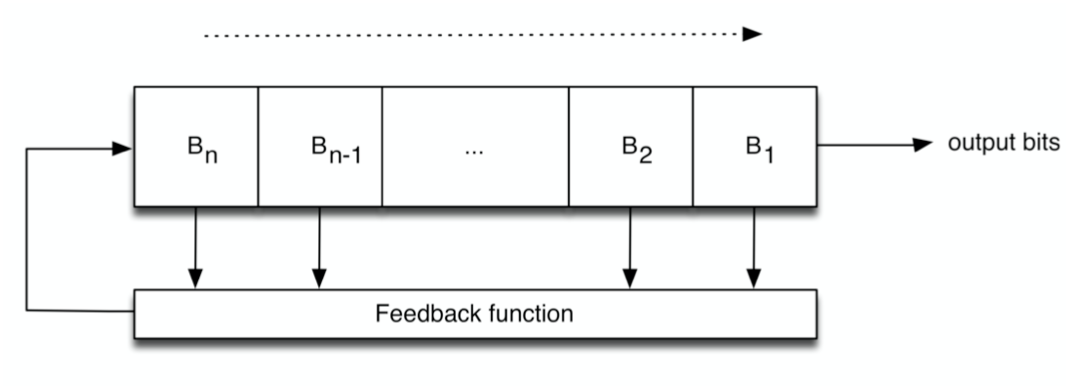
\includegraphics[scale=0.5]{img/img1.png}
\end{wrapfigure}
A LFSR is key stream generator of historical importance. A shift register is a set or register (small memories) next to each other. At every clock-cycle the content of a box is deplaced to the neighboorh. The last box's content is the output. The new value at the beginning is obtained thanks to a feed-back from the bits in the register. For example we could XOR values. It's a linear process because there is only a XOR. It isn't used anymore by itself but it's the basis for a lot of other system.\\
The maximum periodicity is $2^8 - 1$ since there is 8 register, it means we have $2^8 = 256$ configuration possible. The configuration with 0 in every register only gives 0 so it isn't usefull. Thus we can have a maximum stream of 255 bit before the stream repeat itself. So its not bad but also not the most secure system.

\paragraph{Trivium}
Another key stream generator, very fast on hardware and software. Based on LSFR but this time there are XOR and AND so it's not linear. There are 288 register, it use a 80 bits key, the nonce is stocked after, then for 200 cycle the  trivium is "filled", after that we have the first output. Security not broken but they are attacks that work for trivum with less register (less than 200 blanks to fill at the beginning).

\paragraph{RC4}
It output keystream bytes (8 bits at a time). It has a \emph{state} $S \in \mathbb{Z}^{256}_{256}$, an array of 256 \emph{bytes}.\\
First step : initialization ($k \in \mathbb{Z}^{*}_{256}$, contains both key and nonce)\\
\vspace{-6mm}
\begin{verbatim}
for i from 0 to 255 :
	S[i] <- i
j <- 0
for i from 0 to 255 :
	j <- (j + S[i] + k[i mod |k|]) mod 256
	swap values of S[i] and S[j]
\end{verbatim}
at the end $S$ still contains value from 0 to 255 but in a different order. Order of the swap depoend of $k$.
Second step : Keystream generation
\vspace{-6mm}
\begin{verbatim}
i <- 0, j <- 0
loop as long as necessary:
	i <- (i+1) mod 256
	j <- (j+S[i]) mode 256
	swap values of S[i] and S[j]
	s <- S[(S[i] + S[j]) mod 256]
	output s
\end{verbatim}
$i$ increase, $j$ kinda jump around, we swap 2 values then use them to output $s$.\\
This algo is broken. One of the attacks against it is that there is a high bias of $S[2] = 0$

To remember :
\begin{itemize}
\item To properly use a stream cipher, never forget about the nonce.
\item Linear feedback shift registers (LFSRs) have been historically used to design keystream generators thanks to their well-understood mathematical properties. However, they lack non-linearity.
\item Trivium is a modern example of a keystream generator based on non-linear feedback shift registers (NFSRs). Today it is considered secure, although it does not have so much safety margin (in terms of initialization rounds). In addition, cryptanalysis of primitives is done on variants with lower parameters (mainly the number of rounds) than the nominal version.
\item RC4 is an older example of keystream generator. Widely used until fairly recently, it is nowadays considered broken.
\end{itemize}

\section{Block ciphers}
The goal of this section is to define block ciphers and how to use them in modes to build up actual encryption or authentication schemes. We describe the DES and the AES as examples.\\
\\
A \textbf{block cipher} is a mapping $E : \mathbb{Z}_2^n \times \mathbb{Z}_2^m \rightarrow \mathbb{Z}_2^n$ from a secret key $k \in \mathbb{Z}_2^m$ and an input block $x \in \mathbb{Z}_2^n$ to an output block $y = E_k(x) \in \mathbb{Z}_2^n $. For each key $k$, it has an inverse $x = E_k^{-1}(y)$. It's essentially a set of permutation. \textcolor{red}{! it's not an encryption scheme}, (except if the plain text space is $\mathbb{Z}_2^n$ but it's not even IND-CPA secure).\\
Security notions (informally):
\begin{itemize}
\item Pseudo-random permutation (PRP): without knowing the secret key, it should be infeasible for an adversary having access to $E_k(·)$ to distinguish it from a permutation randomly drawn from the set of all permutations on $\mathbb{Z}_2^n$
\item Strong PRP (SPRP): same, but the adversary also gets access to $E^{-1}(·)$
\end{itemize}

\paragraph{DES} \label{sec:DES} acronyme of Data Encryption Standart\\
The mapping is DES$ : \mathbb{Z}_2^{64} \times \mathbb{Z}_2^{56} \rightarrow \mathbb{Z}_2^{64}$.
\begin{center}
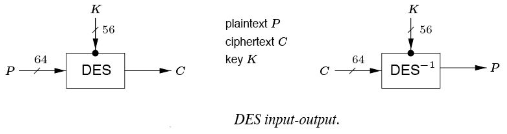
\includegraphics[scale=0.6]{img/img2.png}
\end{center}

\begin{wrapfigure}[19]{l}{2.9cm}
\vspace{-8mm}
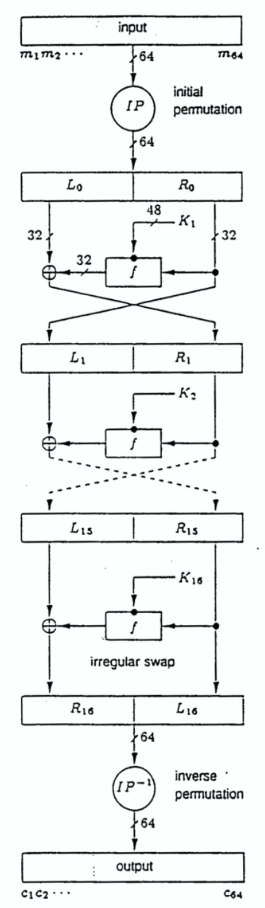
\includegraphics[scale=0.25]{img/img3.png}
\end{wrapfigure}
DES is made in round :\\
An initial bit transposition (IP) is applied to the input: $L_0 \parallel R_0 =$ IP(x), with $L_0, R_0 \in \mathbb{Z}_2^{32}$. Then 16 iterations of the round function:\\
$$L_i = R_{i-1}$$
$$R_i = L_{i-1} \oplus f(R_{i-1},k_i)$$
where $k_1,...,k_{16} \in \mathbb{Z}_2^{48}$ are the sub-keys. The inverse of IP is applied before returning the output: $y = IP^{-1}(R_{16} \parallel L_{16} )$. If we did the round only one time it wouldn't be very secure but doing it 16 times is much better.\\
The first step  (before $L_0 R_0$) is called permutation but it's not a permutation is the sense that we changes all the the bit. It's more a transposition where the bits are change place with other bits in the input.
This structure is called the \textbf{Feistel} network.\\
A round forward is shown above and a round backward is the same thing with the subkeys in reverse order
$$R_{i-1} = L_{i}$$
$$L_{i-1} = R_i \oplus f(L_i,k_i)$$
The main advantages are that $E$  and $E^{-1}$ share the same structure and $f$ don't need to be invertible.\\
\\
The $f$ function is $f : \mathbb{Z}_2^{32} \times \mathbb{Z}_2^{48} \rightarrow \mathbb{Z}_2^{32}$\\
\begin{wrapfigure}[7]{r}{3.4cm}
\vspace{-5mm}
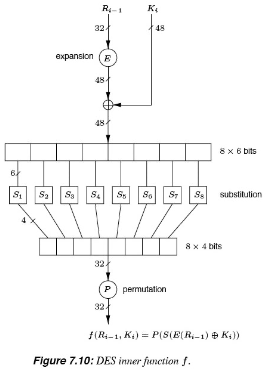
\includegraphics[scale=0.35]{img/img4.png}
\end{wrapfigure}

First expand $R$ through $E$ from 32 to $48 = 16 + 2 \times 16$ bits, compute $E(R) \oplus K_i$, cut in 6-bit blocs $B_j$, $C_j = S_j(B_j)$, 8 different S-Boxes $S_j : \mathbb{Z}_2^6 \rightarrow \mathbb{Z}_2^4$ there to break the linearity, and then do a bit transposition $P : \mathbb{Z}_2^{32} \rightarrow \mathbb{Z}_2^{32}$.
Transposition table exist for $IP, IP^{-1}, E$ and $P$. Similarly, there are table for the S-boxes.\\
\\
\paragraph{Key schedule} : how do we go from a 56-bit key to 16 keys of 48 bits ? We take 48 bits and shuffle them !\\
Secret key : $k \in \mathbb{Z}_2^{56}$\\
First : Bit transposition $C_0 \parallel D_0 = PC1(k)$.\\
Then for $i = 1$ to 16 :\\
	$C_i = L S_i(C_{i-1})$ and $D_i = LS_i(D_{i-1})$,\\ where $LS_i$ is a circular shift to the left by one position when $i=1,2,9,16$ and by two position otherwise\\
	$K_i=PC2(C_i \parallel D_i)$, with PC2 : $\mathbb{Z}_2^{56} \rightarrow \mathbb{Z}_2^{48}$\\
Once again there are table fo $PC1$ and $PC2$.\\
DES has some non-ideal properties : there are 4 weak keys were $E_k$ is an involution i.e. $\forall x E_k(E_k(x)) = x$, 6 pairs of semi-weak keys $(k_1,k_2)$ such that $\forall x E_{k_1}(E_{k_2}(x)) = x$, also there is a complementary property : $E_k(x) = y \Leftrightarrow E_{\overline{k}}(\overline{x}) = \overline{y} $. The complementary property reduces the exhaustive search by one bit.\\
Exhaustive key search in $2^{55}$ is possible with dedicated hardware. But DES security is mostly susceptible to differential and linear cryptanalysis.\\
\\
\textbf{Differential cryptanalysis} analyze the propagation of differences through the round : \\
$f(x) = y$ then $f(\delta \oplus x) = y + \Delta$ where $x$ varies and $\delta$ constant.\\
\textbf{Linear cryptanalysis} analizes the correlation between input and output parities :\\
$\left\vert Pr[v^{\top} x = u^{\top}  f(x)] - \dfrac{1}{2} \right\vert$ where $x$ varies, $u$ and $v$ constant.\\
These 2 technics were applied to DES, now they're test applied to all new block cipher. \\

DES alone is not used anymore but there is an extension called \textbf{Triple-DES}. We use 3 times DES with 3 differents keys !\\
Triple-key triple-DES (168-bit keys) : 3DES$_{k_1 \parallel k_2 \parallel k_3} = $ DES$_{k_3} \circ $ DES$^{-1}_{k_2} \circ $ DES$_{k_1}$\\
The inverse DES$^{-1}$ is there to be retro compatible with single DES : 3DES$_{k \parallel k \parallel k} = $ DES$_{k} \circ $ DES$^{-1}_{k} \circ $ DES$_{k} =$ DES$_k$\\
A Double key triple DES (112-bit keys) also exists : 3DES$_{k_1 \parallel k_2 } = $ DES$_{k_1} \circ $ DES$^{-1}_{k_2} \circ $ DES$_{k_1}$\\

2DES$_{k_1 \parallel k_2 } = $ DES$_{k_2} \circ $ DES$_{k1}$ isn't used because the adversary could encrypt the plain text with all possible $k_1$ and decrypt the corresponding ciphertext with all possible $k_2$ and look for matching in the middle. It would take $2^{57}$ in time and $2^56$ in memory, which is slightly better than single DES but not much better. Also linear and differential analysis are impossible on double DES.\\
\\

\paragraph{Rijndael - AES} is a new type of block ciphers with block size $n = 128$ bits and key size $m = 123, 192 \text{and} 256$ that won the NIST's competion. 3 instance standardized, one for each key size.\\
\begin{tabular}{|c|c|}
\hline
AES-128 : $\mathbb{Z}_2^{128} \times \mathbb{Z}_2^{128} \rightarrow \mathbb{Z}_2^{128}$ & 10 rounds\\
\hline
AES-192 : $\mathbb{Z}_2^{128} \times \mathbb{Z}_2^{192} \rightarrow \mathbb{Z}_2^{128}$ & 12 rounds\\
\hline
AES-256 : $\mathbb{Z}_2^{128} \times \mathbb{Z}_2^{256} \rightarrow \mathbb{Z}_2^{128}$ & 14 rounds\\
\hline
\end{tabular}\\

First the input $x$ of 128 bits is interpreted as 16 \emph{bytes} that can be put into a $4 \times 4$ matrix. Each elements of this matrix is mapped to an other matrix $S$ where each byte $s_{i,j}$ represents an element of the finite field GF$(2^8)$.\\
$$\left(\begin{array}{cccc}
s_{0,0} & s_{0,1} & s_{0,2} & s_{0,3}\\
s_{1,0} & s_{1,1} & s_{1,2} & s_{1,3}\\
s_{2,0} & s_{2,1} & s_{2,2} & s_{2,3}\\
s_{3,0} & s_{3,1} & s_{3,2} & s_{3,3}\\
\end{array}\right) \leftarrow
\left(\begin{array}{cccc}
x_0 & x_4 & x_8 & x_{12} \\
x_1 & x_5 & x_9 & x_{13} \\
x_2 & x_6 & x_{10} & x_{14} \\
x_3 & x_7 & x_{11} & x_{15} \\
\end{array}\right)$$
where $x_i$ is the $i^{th}$ byte of $x$ and vice-versa for the output.\\
GF$(2^8)$ is the Galois Field of size $2^8 = 256$. (see TP 3, Additions are bit wise XOR, multiplication are done modulo $x^8 + x^4 + x^3 + x + 1$ and representation GF(2)[x]/$(x^8 + x^4 + x^3 + x + 1)$ is used).

\textbf{Data path :} (input $x \in \mathbb{Z}_2^{128}$ and $k \in \mathbb{Z}_2^{128 \text{ (or 192 or 256)}}$)
\begin{itemize}
\item Key schedule: $(K_i) \leftarrow $ KeyExpansion($k$)
\item state $\leftarrow x$ (but represented as GF$(2^8)^{4\times 4})$
\item AddRoundKey (state, $K_0$)
\item For each round $i = 1$ to 9 (or 11 or 13)
\begin{itemize}
\item SubBytes(state)
\item ShiftRows(state)
\item MixColumns(state)
\item AddRoundKey(state, $K_i$
\end{itemize}
\item And for the last round :
\begin{itemize}
\item SubBytes(state)
\item ShiftRound(state)
\item AddRoundKey(state, $K_{10\text{ (or 12 or 14)}})$
\end{itemize}
\end{itemize}
Output $y \leftarrow$ state back in $\mathbb{Z}_2^{128}$. Below are the different operation done during a round.
\begin{center}
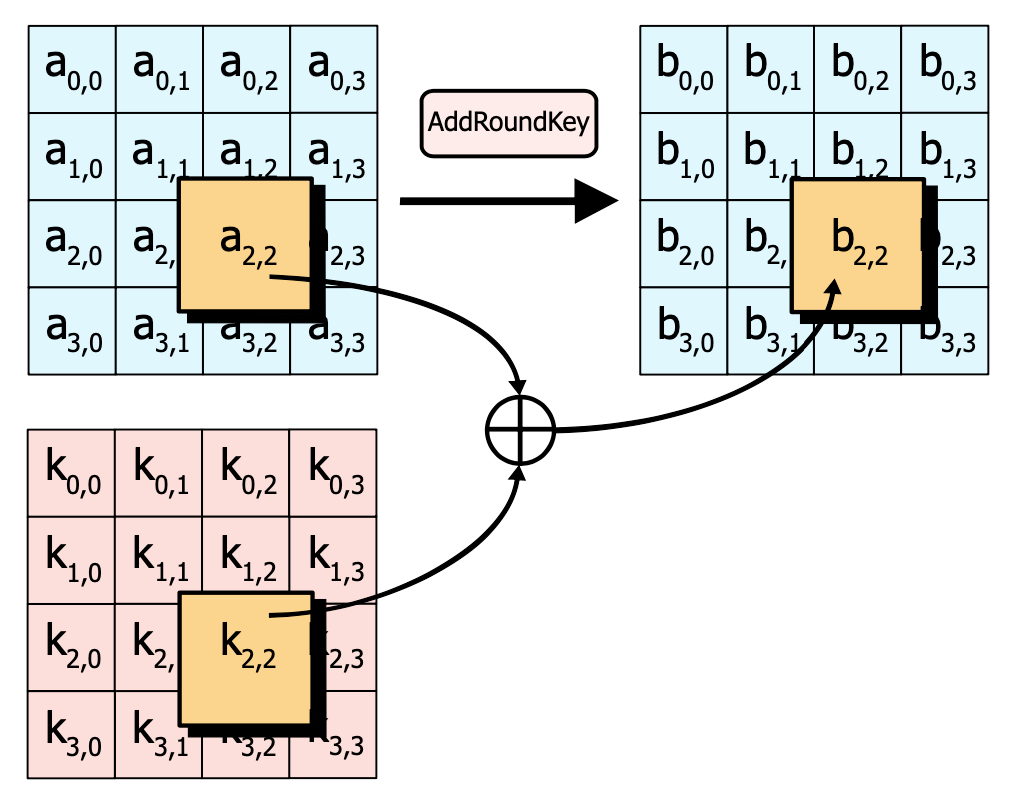
\includegraphics[scale=0.3]{img/img5.png}
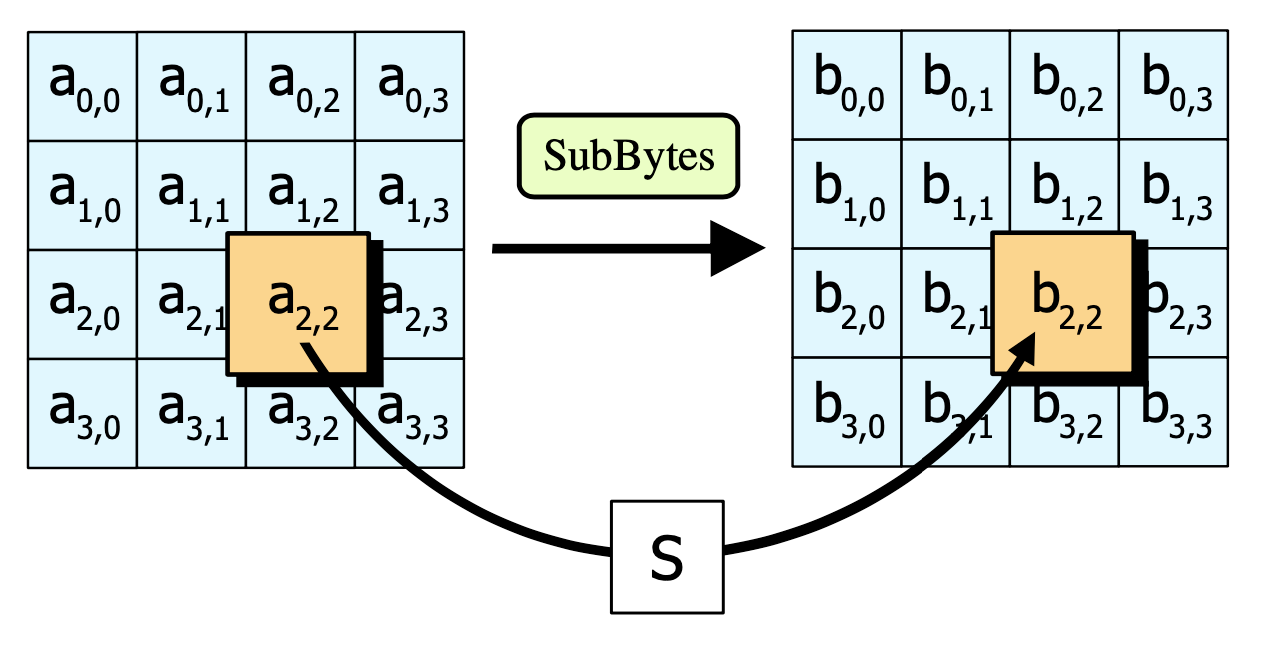
\includegraphics[scale=0.3]{img/img6.png}
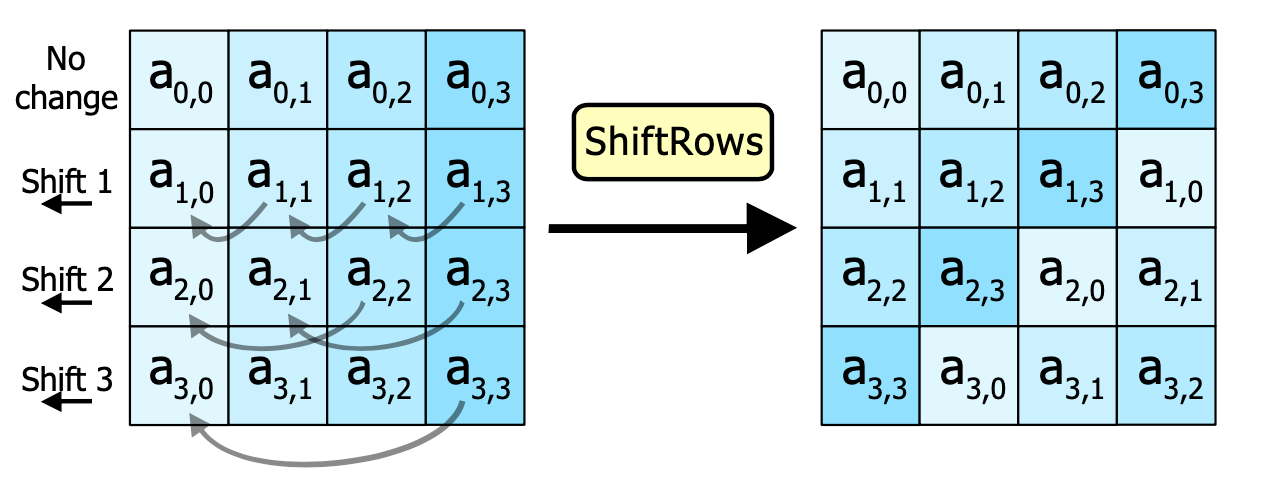
\includegraphics[scale=0.3]{img/img7.png}
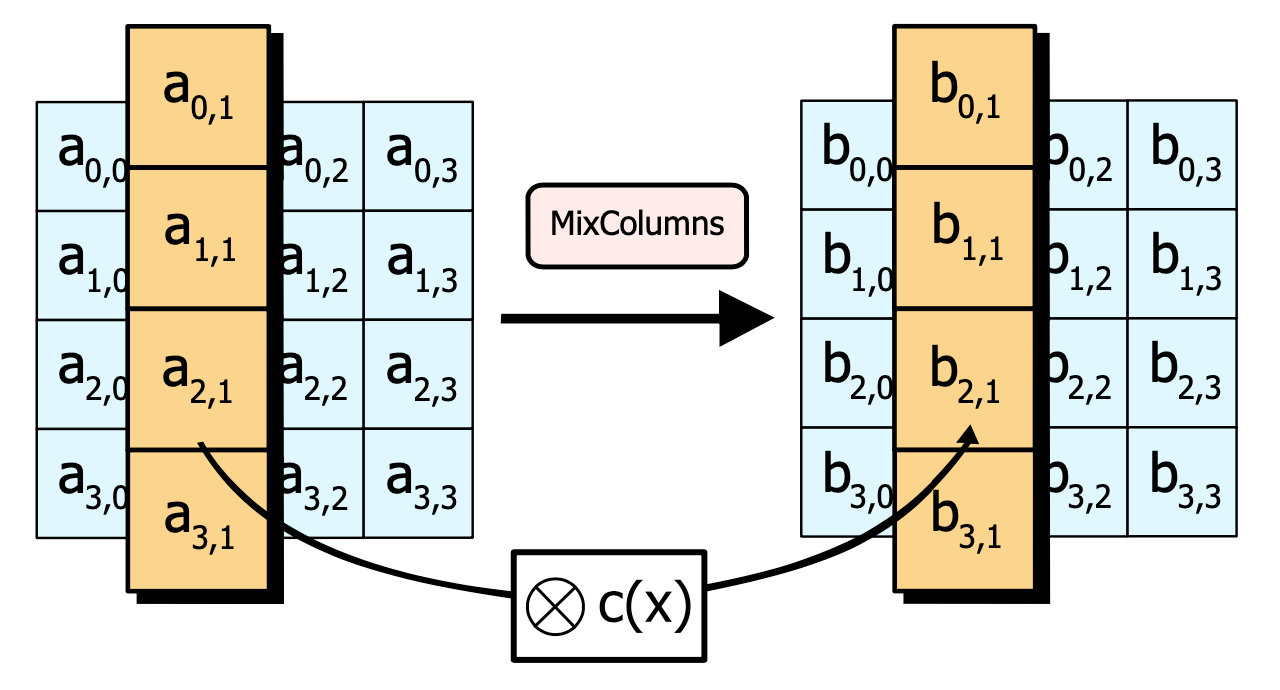
\includegraphics[scale=0.3]{img/img8.png}
\end{center}
SubBytes is the only non-linear operation, the S-box operation is based on the multiplicative inverse in GF($2^8$) (see TP).\\
The MixColumns provides diffusion in the state. We do a matrix multiplication by a given matrix for each colone (The multiplication are done in GF(256)). If we change 1 byte in the input colone, all 4 bytes change in the output. It maximise the propagation of change also called MDS (max distance separation) : $\#$input changed = $\#$output changed = 0 or $\#$input changed + $\#$output changed $\geq$ 5. The multiplication done is\\
$$\left(\begin{array}{c}
b_0 \\ b_1 \\ b_2 \\ b_3
\end{array}\right) = 
\left(\begin{array}{cccc}
x & x+1 & 1 & 1\\  
1 & x & x+1 & 1\\  
1 & 1 & x & x+1\\  
x+1 & 1 & 1 & x\\  
\end{array}\right)\left(\begin{array}{c}
s_0 \\ s_1 \\ s_2 \\ s_3
\end{array}\right)$$
The $4\times 4$ matrix can also be written in hexadecimal format:
$$\left(\begin{array}{cccc}
02 & 03 & 01 & 01\\  
01 & 02 & 03 & 01\\  
01 & 01 & 02 & 03\\  
03 & 01 & 01 & 02\\  
\end{array}\right)$$
The inverse of MixColumns uses the inverse (hexadecimal) matrix:
$$\left(\begin{array}{cccc}
0E & 0B & 0D & 09\\  
09 & 0E & 0B & 0D\\  
0D & 09 & 0E & 0B\\  
0B & 0D & 09 & 0E\\  
\end{array}\right)$$

\textbf{Inverse Data path :} (input $y \in \mathbb{Z}_2^{128}$ and $k \in \mathbb{Z}_2^{128 \text{ (or 192 or 256)}}$)
\begin{itemize}
\item Equivalent key schedule: $(K'_i) \leftarrow $ EqKeyExpansion($k$)
\item state $\leftarrow y$ (but represented as GF$(2^8)^{4\times 4})$
\item AddRoundKey (state, $K'_{10 \text{(or 12 or 14)}}$)
\item For each round $i = $ 9 (or 11 or 13) down to 1:
\begin{itemize}
\item InvSubBytes(state)
\item InvShiftRows(state)
\item InvMixColumns(state)
\item AddRoundKey(state, $K'_i$
\end{itemize}
\item And for the last round :
\begin{itemize}
\item InvSubBytes(state)
\item InvShiftRound(state)
\item InvAddRoundKey(state, $K'_{0})$
\end{itemize}
\end{itemize}
Output $x \leftarrow$ state back in $\mathbb{Z}_2^{128}$.\\
\\
\paragraph{Mode of operation :} They allow us to go from a block cipher to an encryption (authentication) scheme that works for plaintexts (message) of any length.\\

A bad example is the electronic codebook (ECB) where the message is cut into blocks and all blocks are encoded in the same ways $\rightarrow$ Patterns present in the message still appear in the ciphertext.\\

There are several mode of operation, a first one is \textbf{Ciphertext block chaining (CBC)}:
\begin{center}
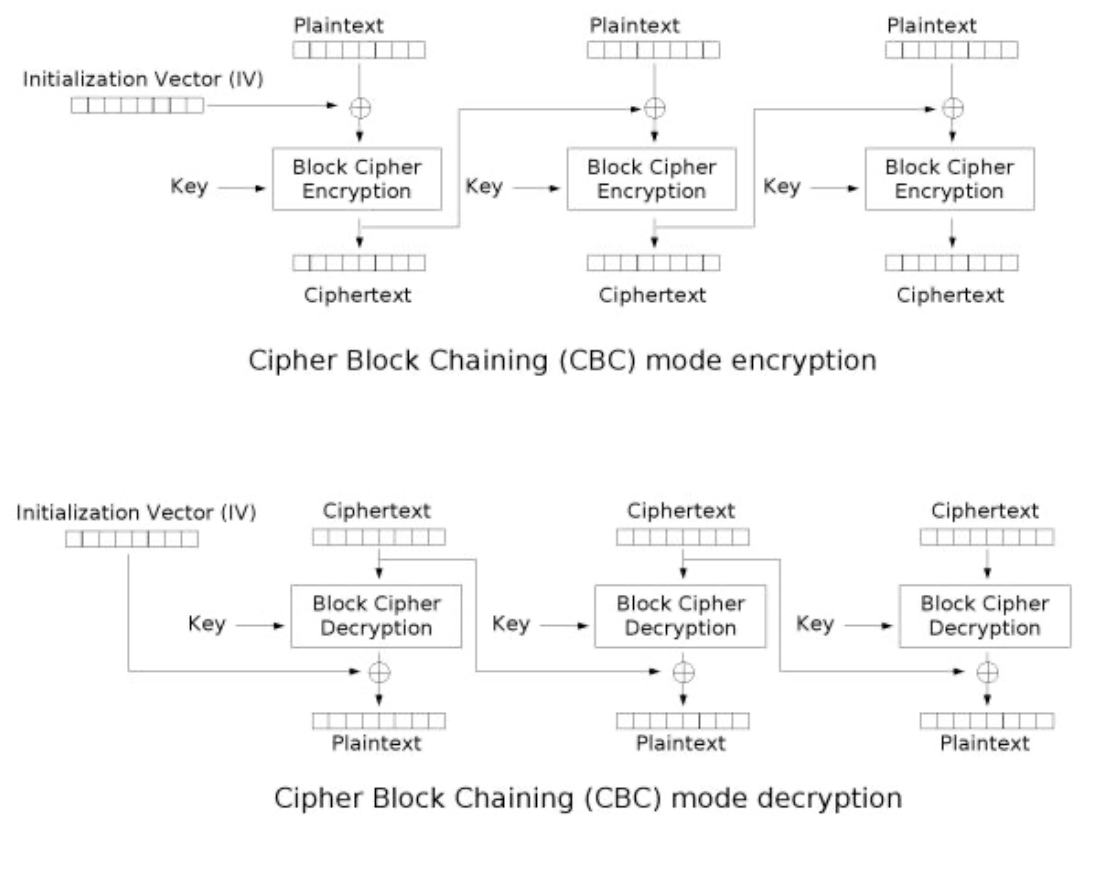
\includegraphics[scale=0.5]{img/img9.png}
\end{center}
The plain text is split into block of the appropriate size for the block cipher used. The output of a block cipher is XORed with the next block of plaintext in order to hide eventual pattern in the plaintext. When we change a bit in the first block of plain text, it's spread. The initialization vector is there to not recognize if the first block is identical in 2 different messages. More formally :\\
Input : secret key $k \in \mathbb{Z}_2^{m}$, plaintext $p \in \mathbb{Z}_2^*$ and nonce $N \in \mathbb{N}$\\
Output : ciphertext $c \in \left(\mathbb{Z}_2^n\right)^*$\\
1) Pad $p$ with 10* and cut into blocks ($p_1, p_2, ...$)\\
2) Define $c_0 = E_k(N)$ (initialization vector is the encryption of the nonce, if we assume the receiver doesn't know the nonce we need to transmit c0) and then for $i \geq 1$
$$c_i = E_k(p_i \oplus c_{i-1})$$
To decrypt:		$p_i = E_k^{-1} (c_i) \oplus c_{i-1}$\\

Limits of CBC : what happens if at some point 2 cyphertext blocks of different messages (or part of the messages), encrypted with the same keys, are the same ?
$$c_i = c'_j$$
$$E_k(p_i \oplus c_{i-1}) = E_k(p'_j \oplus c'_{j-1})$$
$$p_i \oplus c_{i-1} = p'_j \oplus c'_{j-1}$$ 
$$p_i \oplus p'_j = c_{i-1} \oplus c'_{j-1}$$
Which means we know the XOR of the two plaintext $\longrightarrow$ some information about the plaintext is revealed !\\
What is the probability that $c_i = c'_j$. It's the same kind of problem as how many person we need to have 50\% chance of having 2 person with the same birthday ($\longrightarrow$ birthday paradox). The problem here is as such :\\
We have $2^n$ objects and makes $L$ draws with replacements. What value for $L$ in order to have a decent chance to get a collision.\\
\begin{itemize}
\item after $L$ draws there are $\dfrac{L(l-1)}{2} \approx \frac{L^2}{2}$
\item for each pair, the prob of getting the same object is $2^{-n}$
\item so the prob of collision is $\approx \dfrac{L^2}{2}.\dfrac{1}{2^n} = \dfrac{L^2}{2^{n+1}}$
\item when $L = \sqrt{2^n} = 2^{n/2}$, prob $\approx \frac{1}{2}$
\end{itemize}
So prob that $c_i = c'_j$ becomes very likely when the number of blocks encrypted under the same key ($L$) reaches the order of $2^{n/2}$ with $n$ the block size. So it's more a problem for DES ($2^{32}$ blocks) than AES ($2^{64}$ blocks)\\

An other mode of operation is \textbf{Counter (CTR)}, we have as:\\
Input : secret key $k \in \mathbb{Z}_2^m$, plaintext $p \in \mathbb{Z}_2^*$ and nonce $N \in \mathbb{N}$\\
Output : ciphertext $c \in \left(\mathbb{Z}_2^n \right)*$\\
So we pad $p$ with 10* and cut into block $\left( p_1,p_2,...\right)$, generate the keystream $k_i = E_k(N \parallel i)$, where $i$ is the block number, $\longrightarrow c_i = k_i \oplus p_i$\\
To decrypt, generate the same keystream and $p_i = k_i \oplus c_i$ 
\begin{center}
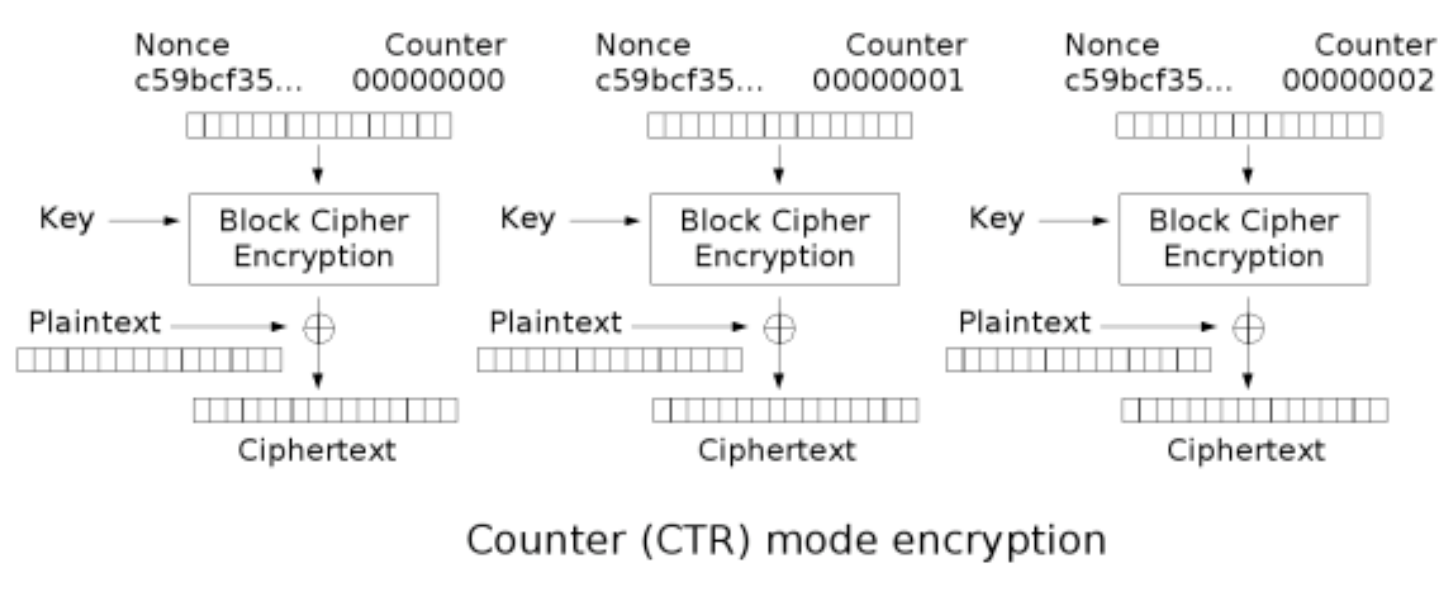
\includegraphics[scale=0.5]{img/img10.png}
\end{center}

Yet another mode of operation is \textbf{CBC-MAC}, it's the only mode of operation we can use to compute a MAC (and thus use for authentication).\\
Input : secret key $k \in \mathbb{Z}_2^m$, message $m \in \mathbb{Z}_2^*$\\
Output : MAC $\in \mathbb{Z}_2^n$\\
Then we prepend (add at the beginning) $m$ with its length, pad len$(m)\parallel m$ with 10* and cut into block $(m_1,m_2,...,m_x)$, define $z_0 = 0^n$ and compute $z_i = E_k(m_i \oplus z_{i-1})$\\
Output MAC $= z_x$
\begin{center}
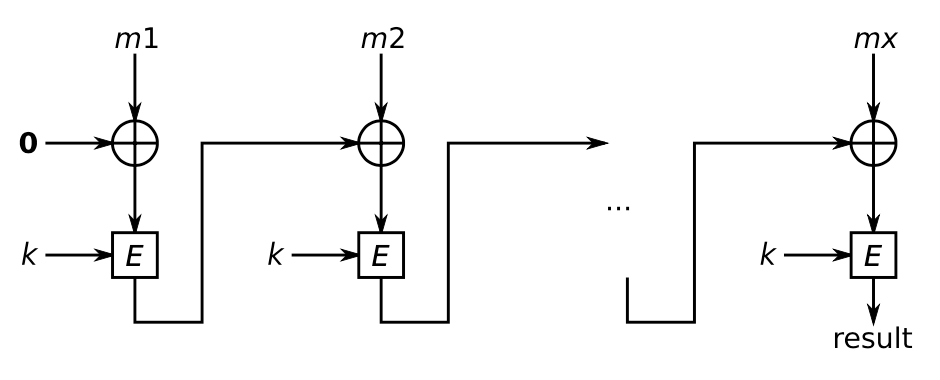
\includegraphics[scale=0.6]{img/img11.png}
\end{center}

To remember:
\begin{itemize}
\item A block ciphers is a primitive, a building block, rather than a small encryption scheme. The use of words "plaintext" and "ciphertext" in the literature to denote the input and output blocks can be misleading.
\item DES is not considered secure nowadays, because of its too small key and also because attacks with lower complexity than the exhaustive key search exist.
\begin{itemize}
\item What is the purpose of each step
\item How to compute the inverse block cipher
\end{itemize}
\item Triple-DES is still considered secure nowadays except for its short block size of 64 bits that limits its use in some modes. $\rightarrow$ Why not use Double-DES?
\item Rijndael, standardized as the AES after an open international competition, is a family of block ciphers that are considered secure nowadays. Today, the AES is ubiquitous in implementations and protocols.
\begin{itemize}
\item What is the purpose of each step
\item What is the MDS property of MixColumns
\item How to compute the inverse block cipher
\end{itemize}
\item CBC and CTR are secure encryption modes. In particular, CTR transforms the block cipher into a keystream generator.
\item CBC-MAC is a secure authentication mode.
\item CBC, CTR and CBC-MAC are limited by the birthday bound in the block size
\end{itemize}


\section{Permutations}
The goal of this section is to define permutations and how to use them in modes to build up actual encryption or authentication schemes. In particular, we focus on sponge and duplex-based modes.\\

A cryptographic \textbf{permutation} is  a bijective (reversible) mapping:
$$f : \mathbb{Z}_2^b \rightarrow \mathbb{Z}_2^b$$
so input block $x \in \mathbb{Z}_2^b$ has $b$ bits and output $y = f(x) \in \mathbb{Z}_2^b$ block too. There is also a inverse $x = f^{-1}(y)$. It's not a permutation bit by bit but for whole set of bits!\\

\begin{wrapfigure}[9]{l}{5.9cm}
\vspace{-8mm}
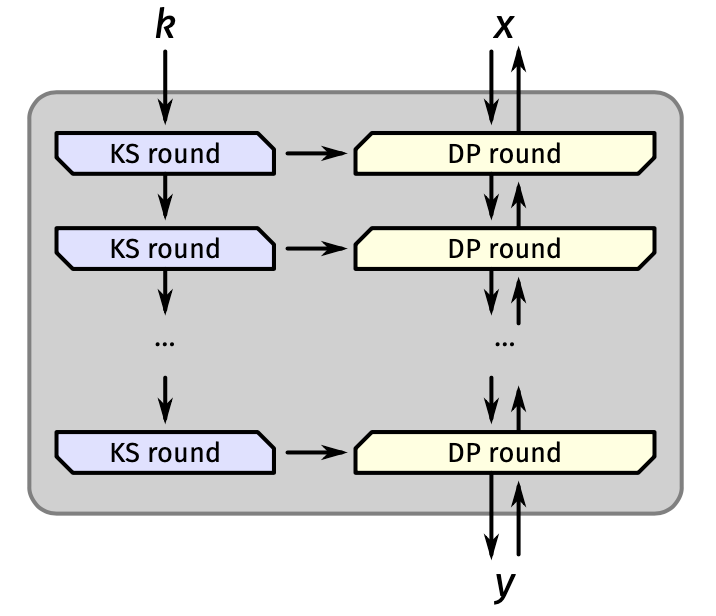
\includegraphics[scale=0.4]{img/img12.png}
\end{wrapfigure}
In block ciphers, we have the input $x$ that undergos several round befor becominf the output $y$, (data path - right), the key $k$ also undergos several round in order to produce the key for each round (key path - left).
There is diffusion from the key to the data but not the other way.\\ 
That condition is necessary if we want to invert invert the path and decrypt. Indeed if we have the last key depending on the input $x$ we can't go from $y$ to find $x$ even with $k$ known.\\
\\

\begin{wrapfigure}[10]{4}{5.9cm}
\vspace{-8mm}
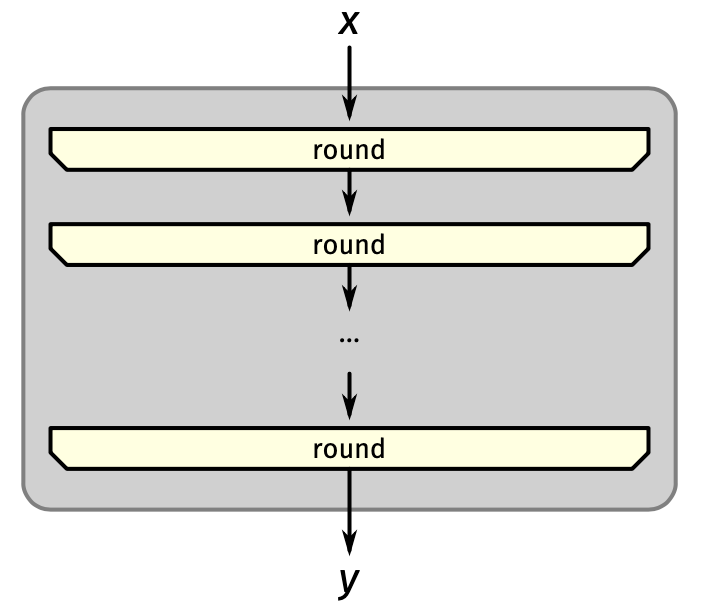
\includegraphics[scale=0.4]{img/img13.png}
\end{wrapfigure}

However, we don't always need to be able to do $y \rightarrow x$, if we don't need to invert then we can have diffusion from the data toward the key. In that case we can even fuse the data path and the key path in a single path were $x$ undergos several round and becomes $y$. We do not care which part are the key and which part are the message but we increase the diffusion. This construction is made from permutations. (it's still invertible as long as we get the whole output)\\

The sponge construction is a mode using permutation, it can have an input $M$ and an output of any size $Z$. It uses a state of $b$ bits (size of our permutation) split into an inner part ($c$) and an outer part ($r$). All bits are sets at 0 at the beginning. The message is padded with 10* so that the length is a mutiple of $r$ and we cut it into block of $r$ bits.\\
The first block is XORed to the outer part then the whole state is permutated then the next block is XORed to r,... untill the whole message has been XORed (absorbing phase). Then we take outer part of the state and that gives us the first $r$ bits of the output, then apply permutation and do again untill we have enough output bits. A sponge function is a concrete instance with a given $f,r,c$.\\
$r$ fixes the speed and $c$ fixes the security.
\begin{center}
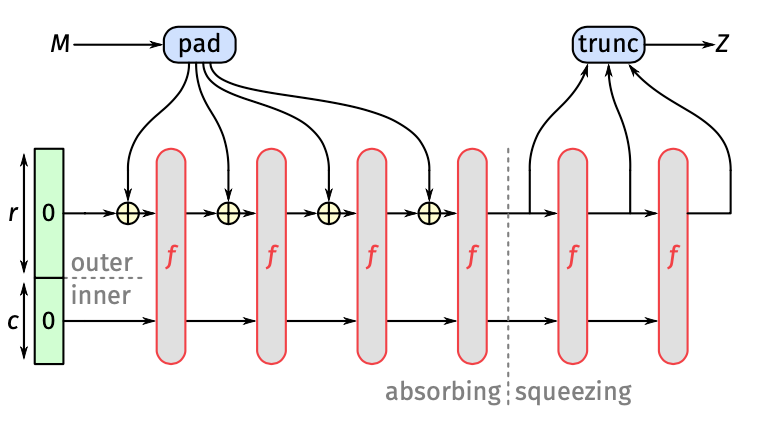
\includegraphics[scale=0.6]{img/img14.png}
\end{center}
More formally : A sponge function implements a mapping from $\mathbb{Z}_2^*$ to $\mathbb{Z}_2^{\infty}$ (truncated at an arbitrary length)\\
\begin{itemize}
\item $s \leftarrow 0^b$
\item $M \parallel 10^*1$ is cut into $r$-bit blocks
\item For each $M_i$ do (absorbing phase)
\begin{itemize}
\item $s \leftarrow s \ominus (M_i\parallel 0^c)$
\item $s \leftarrow  f(s)$
\end{itemize}
\item As long as output is needed do (squeezing phase)
\begin{itemize}
\item Output the first $r$ bits of $s$
\item $s \leftarrow  f(s)$
\end{itemize}
\end{itemize}
To use a sponge function with a key we concatened the key $K$ with the message $M$. It means that the first bits of the state are unknown to the adversary then after a permutation the whole state is unknown to the adversary. When we start squeezing the adversary now know the $r$ first bits of the state. If we had $c = 0$ then in the squeezing phase the adversary would know the whole state between permutation and thus deduce the permutation. That why $c$ determine the security. security strength is $\frac{c}{2}$ bits (it's a birtday bound on the inner part).\\

We can use the keyed sponge as a stream cipher, we just have to conctenate our key and nonce, XOR that to the outer part then do the squezzing phase until we have all the bits wanted for our key stream. $s_i \leftarrow $ sponge$_K$(nonce) produces keystream from key $K$ and nonce.
$$c_i = m_i + s_i \ (\text{in} \mathbb{Z}_2)$$

We can do authenticated encryption with the spongeWrap, it's a variant of the sponge construction where the first XOR is done with a concatenation of the Key and the nonce, then we XOR block of the message and generate a key stream at the same time. The squezzing phase gives us the MAC. SO we have authentication and we can encrypt by XORing the message with the keystream  (of course if we don't encrypted and just produce the MAC then it's an authentication scheme). Formally :
\begin{itemize}
\item Keystream : $s_i \leftarrow$ sponge$_K$(nonce$\parallel$previous plaintext blocks)
\item MAC : sponge$_K$(nonce$\parallel$plaintext)
\end{itemize}

The duplex construction is another construction of similar security strength to the sponge construction. It's a construction where we get an output blocks everytime we "permutate" an input block, so the length of the output is conditionnal to the length of the input. More formally :
\begin{itemize}
\item Object : $D = $ DUPLEX[$f$,pad,$r$]
\item Requesting $l$-bit output $Z = D$.duplexing($\sigma, l$) with input $\sigma$ and output $Z$ limited in length and $Z$ dependent on all previous inputs
\end{itemize}

\begin{center}
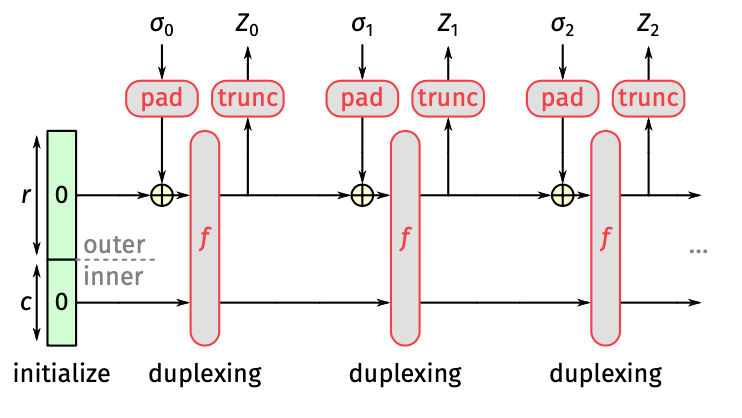
\includegraphics[scale=0.5]{img/img15.png}
\end{center}

Ascon is an exemple of duplex construction used for authenticated encryption. The idea is to put data of the message in 4 row, operation are done on the columns then on the rows independently.\\

To remember:
\begin{itemize}
\item Permutations do not have a dedicated key input. Instead, the input of a permutation can be seen as aggregating the key and block inputs of a block cipher.
\item The keyed sponge construction is a mode of operation that builds a keyed sponge function from a permutation. A keyed sponge function takes as input a secret key and an input string, and produces an output string of user-chosen length.
\begin{itemize}
\item How to do stream encryption using a keyed sponge function.
\item How to compute a MAC using a keyed sponge function.
\end{itemize}
\item The keyed duplex construction is a mode of operation that builds a keyed duplex object from a permutation. A keyed duplex object is useful in that it alternates blocks of input with blocks of output, and this can be exploited to perform authenticated encryption.
\begin{itemize}
\item How to do authenticated encryption using a keyed duplex object.
\end{itemize}
\end{itemize}


\section{Design of symmetric primitive}
This section is an intermezzo where we give more details about the ingredients that are typically used when designing a primitive in symmetric cryptography\\

When talking about DES, we mentionned that transposition and permutation shouldn't be confused. Permutation has been formally define in the previous section, here is the definition of transposition : $\Pi : \mathbb{Z}_2^b \rightarrow \mathbb{Z}_2^b$ with $(x_1,x_2,...x_n) = \Pi(x_{\pi(1)},x_{\pi(2)},...,x_{\pi(n)})$ for some permutation of the bit position $1,...,n$. We keep the same bits but we changes there places !\\

We've talked about linear scheme, here are the relevant definition where $f$ is a function from $\mathbb{Z}_2^n$ to $\mathbb{Z}_2^m$ and $\oplus$ is the bitwise addition modulo 2:\\
The function $f$ is \textbf{linear} iff
$$\forall x,y \in \mathbb{Z}_2^n : f(x\oplus y) = f(x) \oplus f(y)$$
The function $f$ is \textbf{affine} iff
$$\forall x,y \in \mathbb{Z}_2^n : f(x\oplus y) = f(x) \oplus f(y) \oplus f(0^n)$$
Rmq : a linear function is also affine, linear function has only term of degree 1 and affine function has only term of degree 1 or 0.\\
Exemple of linear function : $f(x) = 0$, $f(x,y) = x \oplus y$, bit transposition or a composition of those.\\
Exemple of affine function : $f(x) = x \oplus$ constant; linear functions or a composition of those.\\
Linear are included into affine, linear $\Rightarrow$ affine so it means that non-affine $\Rightarrow$ non-linear. (// with rectangle and square, square $\Rightarrow$ rectangle, not-rectangle $\Rightarrow$ not-square)\\

Diffusion is another usefull notion, let $f$ be a function from $\mathbb{Z}_2^n$ to $\mathbb{Z}_2^m$ : the function $f$ provides \textbf{diffusion} if at least one input bit influences more than one output bit.\\

$\longrightarrow$ In primitives, we often would like that each output bit depends in a complicated (non-linear, non-symmetric) way on all in the input bits.\\
To remember:
\begin{itemize}
\item Do not confuse bit transposition and permutations.
\item What is affinity, linearity, non-linearity.
\item What is diffusion.
\end{itemize}

\section{Authenticated encryption}
This section is an intermezzo with more details about the combination of encryption and authentication in a single primitive.\\

Encryption doesn't imply authentication, anyone could change a bit in the encrypted message, to assure authentication weneed to use a combinaison of the scheme. The best generic method is to encrypt with a key $k_1$ then MAC the ciphertext with key $k_2$, it means we need twice the number of key for the same security level.\\
However they are special mode (using only one key) that combine 2 other modes: CCM combines CTR and CBC-MAC, GCM combines CTR and a ploynomial MAC in GF($2^{128}$),...\\

Definition if authenticated encryption (AE):
\begin{itemize}
\item $M = (A,P)$ \textcolor{ao}{message} with associated data and plaintext
\item $M_c = (A,C)$ \textcolor{red}{cryptogram} with associated data and ciphertext
\item \textbf{wrapping} is $M$ to $M_c$
\item \textbf{unwrapping} is $M_c$ to $M$
\end{itemize}
since we're in symmetric crypto we use the same $k$ for wrapping and unwrapping.\\
For the authentication aspect : unwrapping includes a verification of $M_c$, if not valid, it returns an error $\perp$; the wrap operation adds redundancy so $|C| > |P|$, it's often coded as a tag at the end $C = C'\parallel T$ but not always, sometimes the authentication is mixed with the ciphertext.\\

There are limitation to AE, the adversary can analyze the traffic and see the length and numbers of messages. Usually the length of the cipher is correlated with the length of the plaintext. Solution for these are creating dummy message and adding random length padding of plaintext. But that has to be done at an higher level and the AE scheme security should be independent from that layer.\\

AE is deterministic so $M = M' \Leftrightarrow M_c = M'_c$ which leak informations and rise concern of replay attacks. The solution is to use a nonce $N$, a simple counter suffices.\\
Wrapping : \begin{description}
\item[state] $K$ and past nonces $\mathcal{N}$
\item[input] $M = (N,A,P)$
\item[output] $C$ or $\perp$
\item[processing] if $(N \in \mathcal{N})$ return $\perp$, else add $N$ to $\mathcal{N}$ and return $C \leftarrow \text{Wrap}[k](N,A,P)$
\end{description}
Unwrapping :
\begin{description}
\item[state] $K$
\item[input] $M_c = (N,A,C)$
\item[output] $P$ or $\perp$
\item[processing] return $\text{Unwrap}[K](N,A,C):P$ if valid and $\perp$ otherwise
\end{description}

In case were there is a dialogue, messages have sense in their context so rather than authenticating one message a the time, the tag authenticate all the message before $\rightarrow$ notion of \textbf{session}. It protect against insertion of message of remordering of message in the session.\\
Also we just need a nonce per session, if we have only one session there is no need for nonce, the position of the message is taken into account so sending the same message twice doesn't gives the same cipher.

To remember:
\begin{itemize}
\item It is always possible to combine an encryption and an authentication scheme to get both confidentiality and authenticity. When doing so, the user must use two independent keys, and the best composition method consists in first encrypting then authenticating the ciphertext.
\item By using a dedicated authenticated encryption (AE) scheme, one gets a more efficient scheme than the composition, and one saves key material from using a single key.
\item Encryption does not hide the traffic nor the length of the plaintexts. (Note: not specific to AE.)
\item Authentication necessarily means there is expansion, possibly in the explicit form of a MAC, but not necessarily.
\item In sessions, one authenticates not only individual messages but also the integrity of their sequence.
\end{itemize}

\section{Pseudo-random functions}
The goal of this section is to describe the different secret-key cryptographic functions from a different, more abstract, angle. Some of the modes seen in this chapter can be re-interpreted as a mode on top of a pseudo-random function (PRF).\\

\textbf{Stream-cipher} can be seen as : we use key and nonce in the PRF to produce something random that is then XORed with the plain text to obtain the ciphertext.
\begin{center}
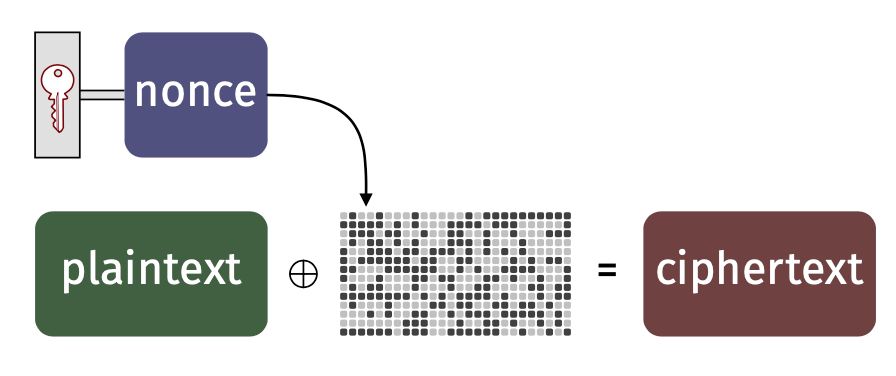
\includegraphics[scale=0.4]{img/img16.png}
\end{center}

\textbf{Message authentication code (MAC)} can be seen as using a PRF with key and plaintext as input and use output as the tag.
\begin{center}
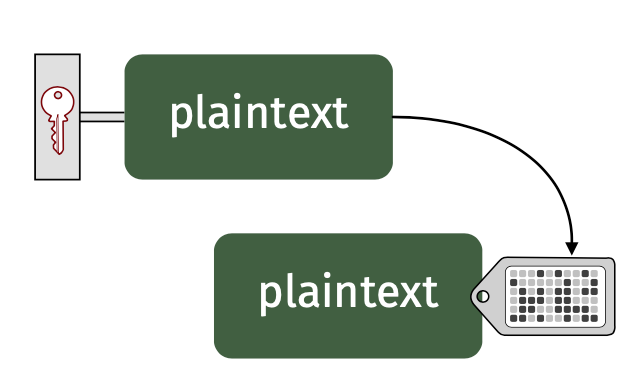
\includegraphics[scale=0.4]{img/img17.png}
\end{center}

For \textbf{Authenticated encryption} we use key and nonce as input of PRF then XOR the output with plaintext to obtain cipher. Then apply PRF on the ciphertext and use the output as the tag of the ciphertext.
\begin{center}
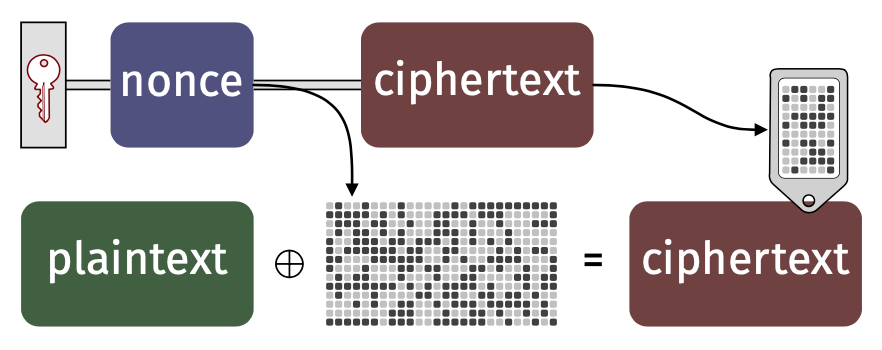
\includegraphics[scale=0.4]{img/img18.png}
\end{center}

\textbf{Incremental MACs} "extends" the PRF. It applies the PRF to a packet  and use the output as the tag, then extend the state with the next packet and use that output as the tag of the new packet. Its the notion of session.
\begin{center}
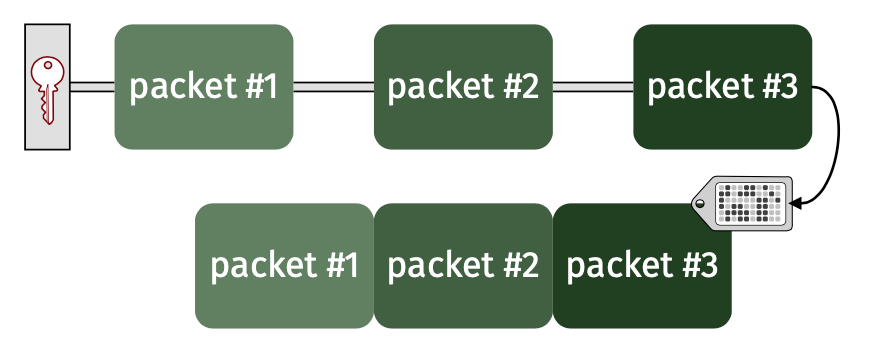
\includegraphics[scale=0.4]{img/img19.png}
\end{center}

To remember:
\begin{itemize}
\item A PRF is a deterministic algorithm that produces a binary string of user-chosen length from a secret key and an input string. From the point of view of an adversary who does not know the key, the output is indistinguishable from unbiased random bits.
\item How a PRF can be used to implement stream encryption, authentication and authenticated encryption.
\end{itemize}

\chapter{Hashing}
\section{Definition and requirements}
The goal of this section is to define what is a hash function or an extendable output function (XOF) and what they are typically used for. We also define what are common requirements and what are the intrinsic security limits.\\
\\
A \textbf{hash function} is defined as $h : {0,1}^* \rightarrow {0,1}^n$, input of any length and output of \emph{fixed} length.\\
A \textbf{output function (XOF)} is a function in which the output can be extended to any length, $h : {0,1}^* \rightarrow {0,1}^{\infty}$.\\
\\
\textbf{Preimage resistance} is the fact that, given $y\in \mathbb{Z}_2^n$, finding $x\in \mathbb{Z}_2^*$ such that $h(x) = y$ should be hard if $h$ is a random function (random oracle). It would need around $2^n$ attempts. \\
\textbf{second preimage resistance} is the fact that, given $x\in \mathbb{Z}_2^*$, finding $x' \neq x$ such that $h(x') = h(x)$ should be hard if $h$ is a random function and need around $2^n$ attempts.(rmq : if the $h$ used isn't second image resistant then it can't be used as a signature because the signature could be forged).\\
\textbf{Collision resistance} is the fact that finding $x_1 \neq x_2$ such that $h(x_1) = h(x_2)$ needs about $2^{n/2}$ attemps if $h$ is a random function.(note : we can't have a bigger exponent because of the probability to draw twice the same thing/ birthday paradox). Property of collision resistance imply second preimage resistance.\\

The list of desired properties is ever-growing but the main objective is that the hash function behave like a \emph{random mapping}.
The requierements above ask that the security strength grows with the output size, it's not very realistic so we usually fix a maximum security $s$ and ask as security requierements for hash or XOF $h$ with $n$-bit output :
\begin{tabular}{|l|l|}
\hline
Preimage resistance & $2^{\min (n,s)}$ \\
Second-preimage resistance & $2^{\min (n,s)}$ \\
Collision resistance & $2^{\min (n/2,s)}$ \\
\hline
\end{tabular}


All practical hash functions are iterated, which means the message $M$ is cut into blocks $M_1,..,M_l$ that are used as input for the function along with $q$ bits of chaining value (CV)(This allow us to determine the size of the input of the function.) The output is the result hash function of the final chaining value.\\
An internal collision would occurs if differents input $M$ and $M^*$ gave the same chaining value. It would means that messages $M \parallel X$ and $M^* \parallel X$ would always collid for any string $X$. 
\begin{center}
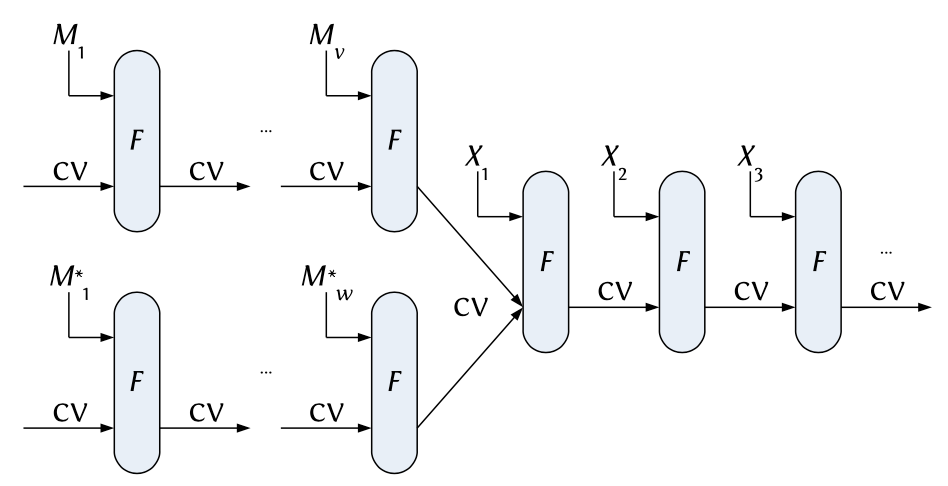
\includegraphics[scale=0.5]{img/img20.png}
\end{center}
The probability of having a internal collision is the probability of having collision in the chaining value. If the chaining value has $k$ bits then the prob is $2^{k/2}$ (birthday paradox). Internal collision becomes as hard to obtain as collision on the output when $s \leq k/2$
This does not occurs in a random mapping !

To remember:
\begin{itemize}
\item A hash function or a XOF does not take a key as input. As a consequence, the attacker can evaluate the digest of any input using only offline computational resources. Note that we can build secret-key schemes by supplying the hash function input with a secret key, but this is not the focus of this chapter.
\item  A hash function or a XOF is a deterministic algorithm. Yet, a good hash function should be such that the output is unpredictable before it is actually evaluated (i.e., there is no shortcut way of knowing what the output will look like). As a consequence, we model the ideal behavior of a hash function as a random oracle. A random oracle (RO) is a non-deterministic algorithm that returns uniformly distributed and independent bits at random for any input value. The only constraint is that the same output bits should be returned when the same value is input.
\item What is the resistance of an ideal hash function, i.e., a RO, against (second) preimage and collision attacks.
\item What is an internal collision and how it puts a limit on the achievable security strength $s$.
\end{itemize}

\section{Zooming from Merkle-Damgård into SHA-1}
This section aims at giving more details into how the "traditional" hash functions (MD4, MD5, SHA-1 and the SHA-2 family) are built. We start from the Merkle-Damgård mode, zoom into Davies-Meyer and finally zoom inside the specific block cipher inside SHA-1.\\
It's the same type of construction as we had with mode and block cipher.

\subsection{Merkle-Damgård}
All function in SHA-1, SHA-2 family use the Merkle-Damgård scheme. It use iteration like we explained before. The chaining value of $n$ bits is initialazed with an initial value that is fixed, The input string is cut into block of $m$ bits and padded. The function used is a compression function that take $m + n$ bits as input and output $n$ bits. Le length of the message is also added at the end of the message, before the padding.
\begin{center}
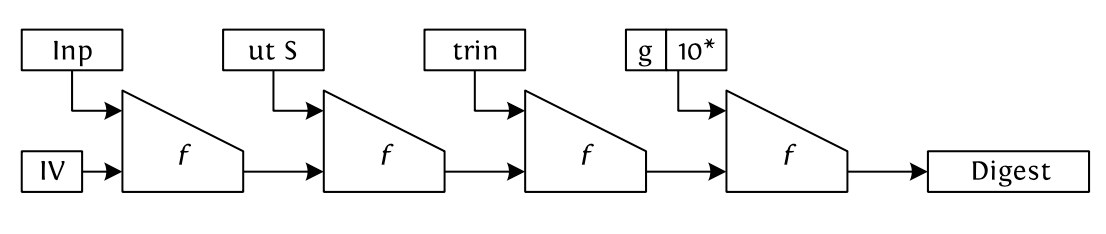
\includegraphics[scale=0.5]{img/img21.png}
\end{center}
MD has the propertie to preserve the collision resistance of the compression function used. However there no preimage or second-preimage resistance.
Note the compression function is not an hash function. The hash function is the whole scheme !
MD also a \textbf{lenght extension} problem,vif we have the digest of an input string $M_1$, then we can compute the digest of some other input string $M_1\parallel ... \parallel M_i$ by using the first digest and just computing the compression function with the rest of the string. \\
$h(M_1) = f(IV,M_1) = CV_1$\\
$h(M_1\parallel ... \parallel M_i) = f(CV_{i-1},M_i) = CV_i$
It's not actually a problem for hash function because nothing absolutly have to stay secret. However if someone want to use MD as an authentication scheme with MAC$(M) = h(Key\parallel M) = CV$, then an adversary can do a forgery with MAC$(M\parallel \text{suffix}) = f(CV\parallel \text{suffix})$ without needing to know the key.\\
The solution is to "nest" the evaluation, it's called HMAC : HMAC$(M) = h(\text{Key}_{out} \parallel h(\text{Key}_{in} \parallel M))$ , then the adversary doesn'have acces to the value $h(\text{Key}_{in}\parallel M )$. It's used a lot but it's just a patch on the defect on MD.


\subsection{Davies-Meyer and other construction using block cipher}
The Davies-Meyer mode of operation build a compression function from a block cipher.
Here the message is put into the key input of the block cipher and the chaining value is put into the data input. The block cipher used are design to be used into hashing function. 
\begin{center}
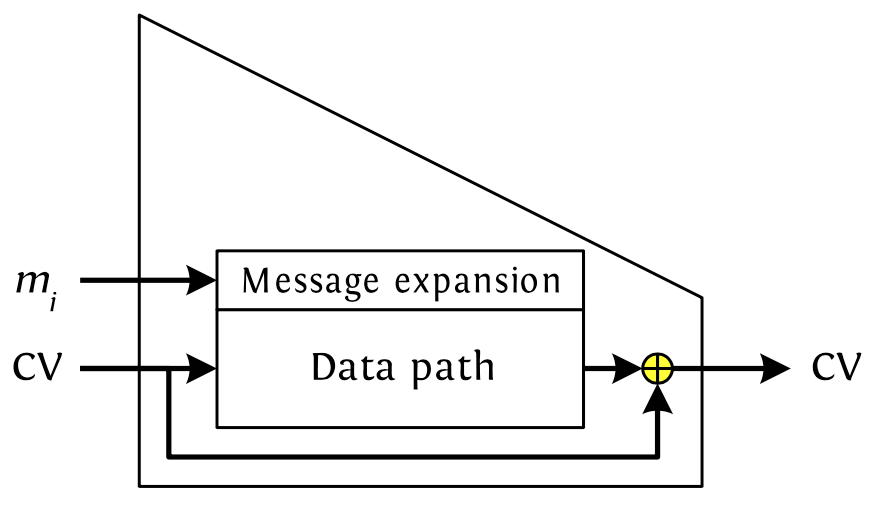
\includegraphics[scale=0.5]{img/img22.png}
\end{center}
The XOR is there to be sure that someone can't fix the CV output then fixe the $m$ (key) invert the block cipher and find an CV input, then repeat the process with a different $m$ and find a collision.\\
\\
Below are other exemple of construction using block ciphers :
\begin{center}
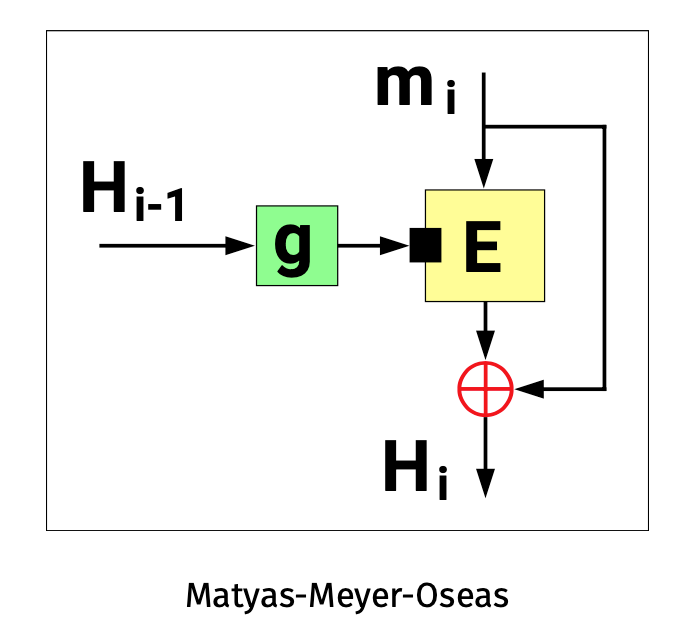
\includegraphics[scale=0.3]{img/img23.png}
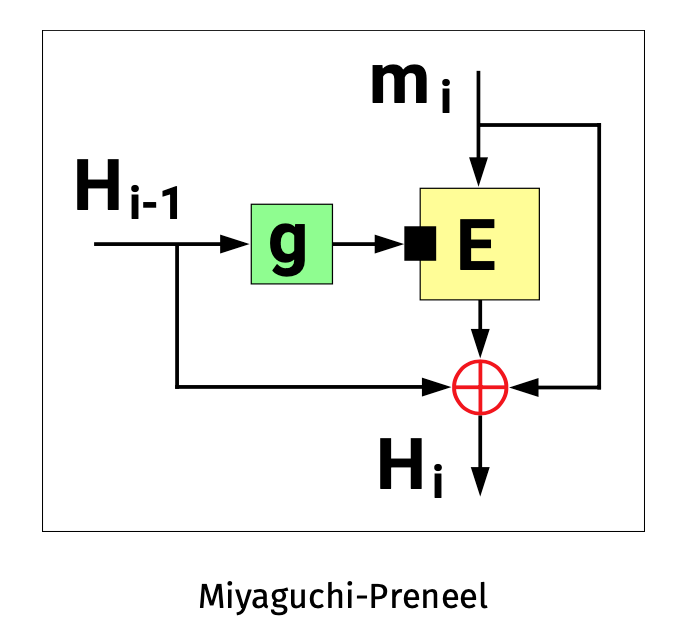
\includegraphics[scale=0.3]{img/img24.png}
\end{center}
The black square represent the key input.

\subsection{SHA-1}
SHA-1 uses Davies-Meyer with a data path of $n = 160 = 5 \times 32$ bits and  a message expansion of $m = 512 = 16 \times 32$ bits. The IV (initial value for chaining value) is predefined (5 number in hexadecimal, at slide 19/45). The data path has 80 steps and thus the message block ($w_0,...,w_{15}$) is expanded as $w_t = (w_{t-3} \oplus w_{t-8} \oplus w_{t-14} \oplus w_{t-16} \lll 1 \ \ (16 \leq t \leq 79)$. The rotation of 1 bit to the left is the only difference between SHA-1 and SHA-0.\\

The data path inside SHA-1 is an unbalanced feisel-network.\\ 
A first collision has been found in 2017 for SHA-1, there exist SHA-1$(P \parallel M_1^{(1)} \parallel M_2^{(1)} \parallel S)=$ SHA-1$(P \parallel M_1^{(2)} \parallel M_2^{(2)} \parallel S)$.
Today there are concrete exemple of collision for MD4, MD5 and SHA-1.\\

SHA-2 looks a lot like SHA-1 but there are a few improvement and so it's not broken. There are 2 compression function in SHA-2 : \\
SHA-{224,256}: $n = 256 = 8 \times 32$ and $m = 512 = 16 \times 32$\\
SHA-{384,512}: $n = 512 = 8 \times 64$ and $m = 1024 = 16 \times 64$\\
Then the message expansion is non-linear contrary to SHA-1 and the mixing is also stronger in SHA-2

To remember:
\begin{itemize}
\item The Merkle-Damgård (MD) mode builds a (variable input length) hash function from a fixed input length hash function (a.k.a. a compression function). The collision resistance of the compression function implies that of the hash function.
\item What is the length extension weakness and why we need HMAC as a patch.
\item What is Davies-Meyer (DM) and why it needs a feed-forward.
\item What is today's status on MD4, MD5 and SHA-1.
\item How SHA-2 improves SHA-1.
\end{itemize}

\section{Modern generic security}
The goal of this section is to give an idea on how the generic (=mode-level) security of hash function is defined nowadays. We give the sponge construction as an example of a permutation-based mode that meets state-of-the-art security notions.\\

In modern hash function it's impossible to prove that a hash function is secure or not secure, like for block ciphers, the only way is to do cryptanalysis and hope no one will find an attack. But we can check if the mode is a good mode (MD is bad because of lenght extension).\\
\begin{wrapfigure}[6]{l}{4.5cm}
\vspace{-8mm}
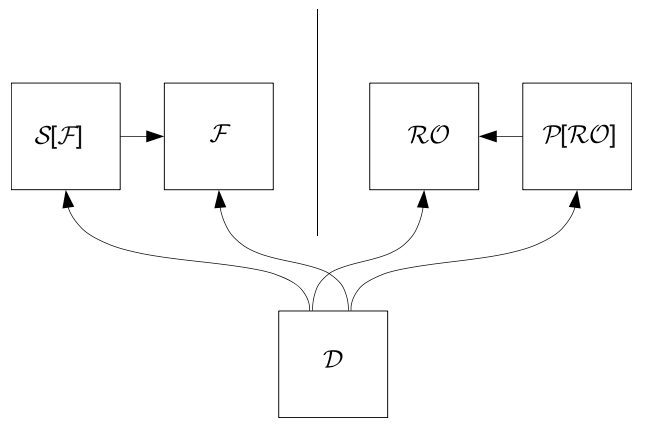
\includegraphics[scale=0.4]{img/img25.png}
\end{wrapfigure}
We want our mode to have \textbf{indifferentialibility}. It means we want a differenciator $D$ to be unable to differenciate between a mode $S[F]$ of a primitive/block cipher $F$ and a random oracl $RO$ (an additional interface is added to the random oracle in order to have the same structure on both side). $D$ has access to the primitive and to the mode ! So the object is to not be able to distinguish between something ideal (RO) and something real ($S[F]$).\\

The consequence of indifferentiability is that the probability any attacks on a concrete hash function suceed is at most the probability the attack succeed on a random oracle added to the probability of distinguishing  the mode from a random oracle.\\
The limitiations of indifferentiability are that it only concern the mode, there is no security proof for the primitive and it's only for single-stage games.\\
\\
We can make Merkle-Damgård indifferentiable by adding a last compression where we use the $CV$ as if it was the message input :
\begin{center}
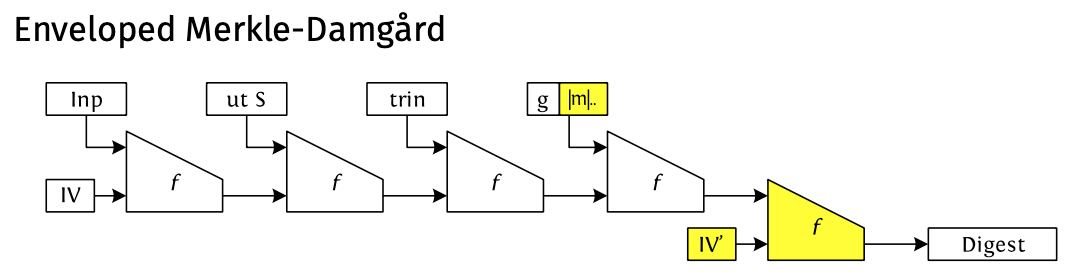
\includegraphics[scale=0.4]{img/img26.png}
\end{center}
We can also use version of the MD above, with a nonce place between the end of the input string and the length of the message, then concataned the result to obtain a mask in order to have a MD suitable for XOF.\\
\\
Another mode that can be used with good indifferentiability properties is the \textbf{sponge construction}
\begin{center}
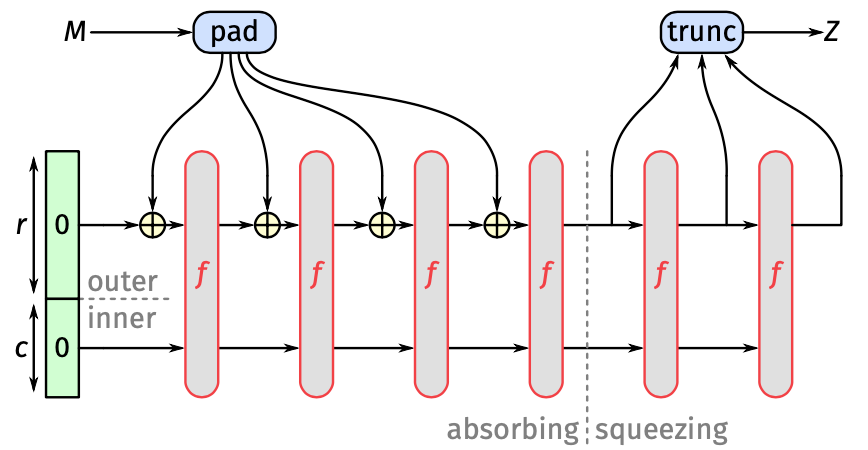
\includegraphics[scale=0.5]{img/img27.png}
\end{center}
This mode of operation natively inplement a XOF, so it can do hashing for any output size. And it's indistinguishable with an advantage of Adv $\leq \dfrac{t^2}{2^{c+1}}$ where $t$ is the time complexity and $c$ the capacity. The advantage becomes non-negligible when $2^{c+1} < t^2$.
The resistance is : 
\begin{center}
\begin{tabular}{|l|l|}
\hline
Preimage resistance & $2^{\min (n,c/2)}$\\
Second-preimage resistance & $2^{\min (n,c/2)}$\\
Collision resistance & $2^{\min (n/2,c/2)}$\\
Any other attacks & $2^{\min (\mathcal{RO},c/2)}$\\
\hline
\end{tabular}
\end{center}

To remember:
\begin{itemize}
\item Keeping the RO as our model, the probability of success of an attack against a concrete hash function can be upper bounded as the sum of the probability that this attack succeeds on the RO and that the concrete hash function can be distinguished from a RO.
\item One can prove that a mode yields something indistinguishable from a RO, but this assumes an ideal primitive (e.g., block cipher or permutation), so this does not prove the security of a concrete hash function. Still, it can exclude flaws in the mode.
\item What is the sponge construction, what is the probability that it can be distinguished from a RO, and how.
\end{itemize}

\section{Inside SHA-3 and beyond SHA-3}
This section describes the inner workings of Keccak sponge function on which the SHA-3 standard is defined. Here we will clarify how the permutation fonction work (\textcolor{red}{! D'après l'assistant le prof aime bien demandé keccak à l'exam vu que c'est son algo !}).\\

Actually Keccak-$f$ is not one permuation but 7 differents permutation with 25, 50, 100, 200, 400, 800, 1600 bits. The smallest one aren't usefull for actual crypto (security too low) but there a small model to test attacks.\\
A permutation is represented as a 3D state, 8 slices of 5x5 bits for the 200 bits permutation. 
\begin{center}
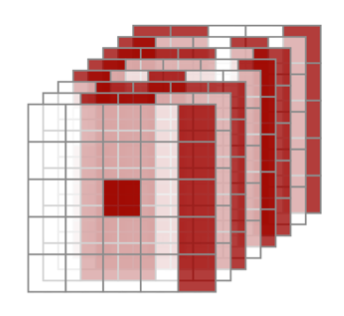
\includegraphics[scale=0.5]{img/img28.png}
\end{center}
The Keccak permutation is composed of 5 steps : 

\paragraph{$\chi$}, the non-linear mapping. \\
It works a bit like an S-box however it's not a list of value but boolean operation on the bits. It maps 5 bits to 5 bits and operate independently an in parallel on 5-bit rows. It flip a bit if the neighbours on the right have 01 pattern. It's cheap !

\paragraph{$\theta$}, mixing bits.\\
It compute the parity $c_{x,z}$ of each column then add to each cell the parity of the neighboring columns : $b_{x,y,z} = a_{x,y,z} \oplus c_{x-1,z} \oplus c_{x+1,z-1}$. It's cheap !
\begin{center}
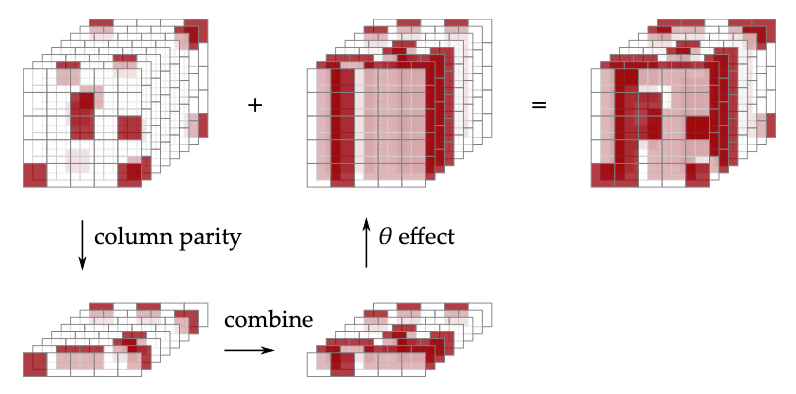
\includegraphics[scale=0.5]{img/img29.png}
\end{center}
It has great diffusion, if we have 1 bits that change, it's going to affect 11 bits after the operation $\theta$. However if we change 2 bits in a columns then the parity doesn't change and $\theta$ doesn't change the output.

\paragraph{$\rho$} fo inter-slice dispersion.\\
$\theta$ only provides diffusion between neighbouring slices. Here we do circular shift on the manes with differents amounts.
\begin{center}
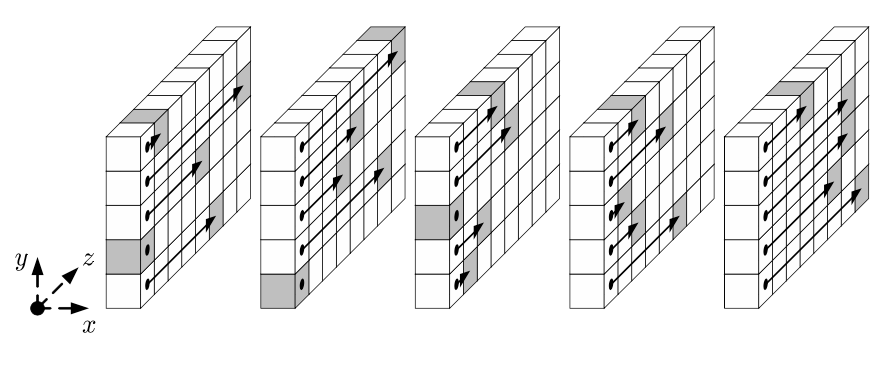
\includegraphics[scale=0.5]{img/img30.png}
\end{center}

\paragraph{$\pi$} for disturbing horizontal/vertical alignement.\\
Here the center of the slides don't  move, the rest rotates in some way\\ $a_{x,y} \leftarrow a_{x',y'}$ with $\left(\begin{array}{c}
x \\ y
\end{array}\right) = \left(\begin{array}{cc}
0&1 \\ 2&3
\end{array}\right) \left(\begin{array}{c}
x' \\ y'
\end{array}\right)$
\begin{center}
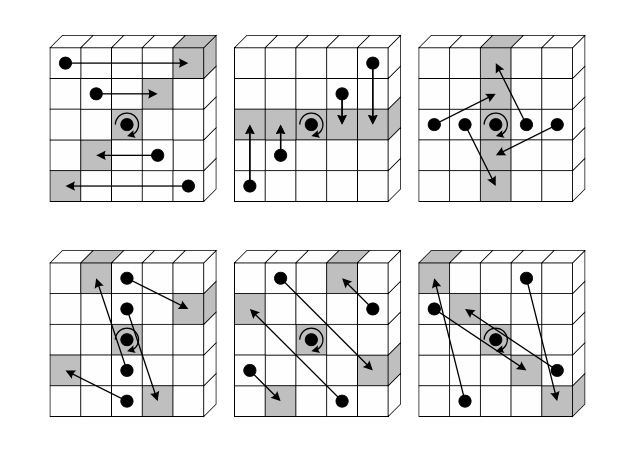
\includegraphics[scale=0.5]{img/img31.png}
\end{center}

\paragraph{$\iota$} to break the symmetry.\\
It's XOR of round-dependent constant to lane in origin. It assures that the round aren't all the same or symmetric and that we don't get fixed point.\\
\\

The round function in keccak is $R = \iota \circ \chi \circ \pi \circ \rho \circ \theta$ and the number of rounds is $12 + 2l$ where $l$ is 0 for 25 bits, 1 for 50 bits, 2 for 100 bits, ... till 6 for 1600 bits.\\
\\

The FIPS 202 standard define 2 XOF functions and 4 drop-in replacemets to SHA-2.
\begin{center}
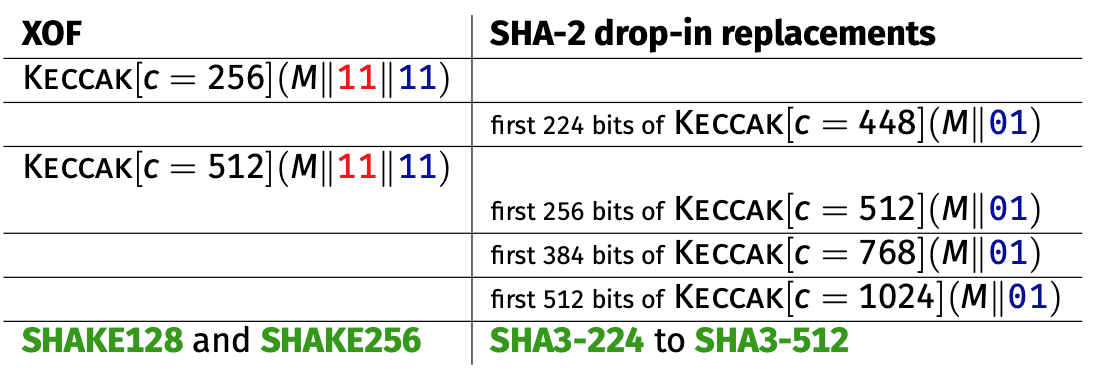
\includegraphics[scale=0.5]{img/img32.png}
\end{center}
SHAKE128 is Keccak with capacity of 256 bits and security level of 128.\\ SHAKE256 is Keccak with capacity of 512 bits and securiyt level of 256. \\
The sufix in red and blue are there for domain separation with SHA3-256 and SHA3-512. When the capacity is different there is automatically domain separation so we don't need to assign special value to distinguish between SHAKE128 and SHAKE256.\\
The security level of Keccak is half the capacity.\\

To have a fast hashing, we can use parallel hash. Also the number of round of Keccak can be cut in half and it would still be secure. So it's a bit over-engineered and could go faster will still being secure with less round.

To remember:
\begin{itemize}
\item Keccak is a family of sponde functions $\longrightarrow$ what is the capacity chosen for the different functions (from SHAKE128 to SHA3-512) in the FIPS 202 standard and why.
\item Keccak-f is a family of 7 permutation $\longrightarrow$ what is the purpose of each step.
\end{itemize}

\chapter{Public-key techniques}

\section{Going public}
The purpose of this section is to highlight the boundaries of public-key cryptography, with a particular stress on the question how to bind a public key with an identity.

A brief reminder, for confidentiality we encrypt the message with the \textcolor{ao}{public} key $k_E$ and decrypt it with the \textcolor{red}{private} $k_D$. It means the encryption key is easier to share and everyone can encrypt. For authenticity we use the \textcolor{red}{private} key $k_A$ to tag the message and the \textcolor{ao}{public} key $k_V$ to check the message tag. If $k_A = k_V$ then it's a MAC, else it's a \emph{signature}. A signature can be verified by anyone.\\

Publics keys are susceptible to \emph{man-in-the-middle attack} where an attacker M put itself between A and B. A gets M's public key and thinks it belongs to B, B gets M's public key and thinks it belongs to A. It means M can decrypt en re-encrypt at will $\Longrightarrow$ we should always check that the public key beling to the right person. To bind a public key to an identity we can either use certificates and public-key infrastructure (PKI, the most used) or use a web of thrust.\\

\paragraph{Public key certificate} binds a public key with identity of its owner. It contains at least the public key, information for identifying its owner, a digital signature on the key and the info. It's also signed by a certification authority. Browsers have the public key of certification authorities and can see if the site they want to access has a certificate.\\
There is a certificate hierarchy between the authority.

\paragraph{Web of trust} use manual key verification over an authentic channel, it compares compare the "fingerprint" (hash function) and if it's correct sign it. The public key are distributed with their signature. We consider a key trustworthy if we signed the key ourselves or if it's signed by someone we trust. In this context, someone we trust is someone where we trust their public key \underline{and} we trust that they do the correct verification.\\

There is different kind of public-key algorithm, here we will see 2 of them : factorization and discrete logarithm problem (modular eponentiation and elliptic curve). Rmq : those method are hard to break on classical computer, with quantum computer they would become easily breakable.\\

The best practice is to use hybrid encryption, meaning combine symmetric and asymmetric encryption. To do so we have A that want to send the encryption $c$ of a message $m$ to B, B has a public key $k_P$.\\
A choose randomly a symmetric key $k$ then comput $(c_k, c_m) = (Enc_{k_P}(k), Enc_k (m))$. Then to decrypt, B first recover the random symmetric key  $k = Dec_{k_P}(c_k)$ then use it to recover $m = Dec_k (c_m)$.\\
\\
To remember:
\begin{itemize}
\item The origin of a public key has always to be questioned, as it can belong to an attacker as in a man-in-the-middle attack.
\item PKI and web of trust are solutions, but be aware of their limits and of their underlying assumptions.
\item The mathematical problems (factoring, discrete logarithm), on which are based the schemes we will see in the course, are relatively easy to break with a quantum computer. Schemes based on other mathematical problems are preferred for the "post-quantum era", but this is not for this course.
\item Hybrid encryption is the best way to take the best of public-key and secret-key techniques.
\end{itemize}

\section{Mathematical background}
This section introduces the different notions that will be needed for the subsequent sections.\\

\subsection{Primes} 
We will use primes number a lot. Proof by contradiction that there are infinitely many primes :\\
Let $p_1=2 < p_2 = 3 < ... < p_r$ be all the existing primes. Let's have $P = p_1 p_2 ... p_r + 1$, $P$ cannot be a prime so we have $p \neq 1$ be one of the existing primes that divides $P$. But $p$ can't be any of $p_1,p_2,...,p_r$ because it would mean $p$ divide the difference between $P - p_1 p_2...p_r =1$ so we would have $p=1$. This means $p$ is a another prime and $p_1,p_2,...,p_r$ aren't all the existing primes.

\subsection{Groups}
It's a set $G$ along with a binary operation $\circ$ that satisfy 4 properties:
\begin{description}
\item[closure] $\forall g,h \in G, g \circ h \in G$
\item[associativity] $\forall g_1,g_2,g_3 \in G, (g_1 \circ g_2) \circ g_3 = g_1 \circ (g_2 \circ g_3)$
\item[identity] there exist an identity $e \in G$ such that $\forall g \in G, e \circ g = g \circ e = g$, $e$ is the neutral element of the group
\item[inverse] $\forall g \in G$, there exists $h \in G$ such that $g \circ h = h \circ g = e$
\end{description}

The \textbf{order} of an element $a$ of a groupe $G$ is the smallest positive integer $m = ord(a)$ such that $[m]a = e$ where $[m]a = a \circ a \circ ... \circ a$ denotes the group operation applied $m$ times to $a$. The order of element represent the number of times it must be combined with itself to get back to the identity.\\
There is a theorem : for any $a$, ots order ord($a$) divides the size $|G|$ of the group.\\
An element $g$ is a \textbf{generator} of $G$ if ord$(g) = |G|$, also a generator can be used to generate all the elements of the group.

\subsection{Modulo}
it's a binary operation : $a \mod n = r$ iff $a = qn + r$ and $0 \leq r \leq n$ ; and an equivalence relation : $a \equiv b \mod n$ iff $\exists k \in \mathbb{Z}$ such that $(a - b) = kn $ or iff $(a \mod n) = (b \mod n)$\\

\textbf{Modular arithmetic} is arithmetic operations where we only care about equivalence modulo some foxed integer $n$.\\
For example the group $\mathbb{Z}_n ,+$ is the set ${0,1,...,n-1}$ with addition modulo $n$. The identity is 0 and the inverse of $x$ is $-x \mod n$, 1 is a generator because all the element can be obtained by adding 1 to itself enough times.

\subsection{Greatest common divisor}
Bezout : For any positive integers $a$ and $b$, there exist integer $x$ and $y$ such that $ax + by =$ gcd$(a,b)$, where gcd$(a,b)$ is the greatest common divisor of $a$ and $b$.\\
Let $S = {ax + by : x,y \in \mathbb{Z}}$ and $d = \min (S \cap \mathbb{N}_{>0})$. Divide $a$ by $d : a = qd + r$ with $0 \leq r \leq d$\\
But $r = a - qd = a -q(ax+by) = (1 - qx)a - (qy)b$ so $r \in S$ and $r < d$ hence $r = 0$ and $d$ divides $a$.\\
Similarly, $d$ divides $b$ and therefore $d$ divides gcd$(a,b)$.\\
The corollary is that $a$ and $b$ are relatively prime (or gcbd$(a,b) = 1$) iff there exist integer $x$ and $y$ such that $ax + by = 1$.

\subsection{Modular multiplication and multiplicative inversion}
The group $\mathbb{Z}_n^*,\times$ is the set ${x : 0 < x <n \text{nad gcd}(x,n) = 1}$ together with multiplication modulo $n$. The identity is 1 and the inverse of $x$ is denoted $x^{-1} \mod n$ and is such that $x^{-1}x \equiv 1 \mod n$. Note : $^{-1}$ is not the usual operation. The inverse $x^{-1}$ exists and is unique iff gcd$(x,n) = 1$. Proves : \\
\begin{description}
\item[$\Rightarrow$ :]$xy \equiv 1 \mod n$ means that $xy = 1 +kn$ for some integer $k$, so $xy + kn = 1$ and gcd$(x,n) = 1$
\item[$\Leftarrow$ :] gcd$(x,n) = 1$ implies that there exist integers $y$ and $z$ such that $yx + zn = 1$, so $xy = 1 - zn$ and $xy \equiv 1 \mod n$. 
\end{description} 

\subsection{Euler's function}
We note the euler's function $\Phi (n)$ the number of integers smaller than $n$ and that are relatively prime with $n$. So $| \mathbb{Z}_n^* | = \Phi(n)$. The formule is :
$$\Phi (n) = n . \prod\limits_{i=1}^r \left( 1 - \frac{1}{p_i} \right)$$
with $n = \prod\limits_{i=1}^r p_i^{e_i}$ for distinct primes $p_1,...,p_r$.\\
Usually to compute $\Phi(n)$ we uses rules dealing with particular cases :
\begin{itemize}
\item Prime $p = \Phi(p) = p-1$
\item Product of 2 distinct primes $p$ and $q$ : $\Phi(pq) = (p-1)(q-1)$
\end{itemize}
Several theorems use Euler's function :\\
\paragraph{Fermat's little theorem} : let $p$ be a prime and $a$ an integer not a multiple of $p$, then $a^{p-1} \equiv 1 \mod p$.
\paragraph{Euler's Theorem} :let $a$ and $n$ two relatively prime integers, then $a^{\Phi(n)} \equiv 1 \mod n$.\\
The consequence is that when we have an exponentiation, it can always be reduced modulo $\Phi(n)$ : $a^e \equiv a^{e \mod \Phi(n)} \mod n$.\\
\textcolor{red}{This will be usefull for the TP}\\

The group $\mathbb{Z}_n^*$ has size $\Phi(n)$, so the generator is an element with ord$(g) = \Phi(n)$. Such a generator exists when$n$ is $2,4,p^a$ or $2p^a$ with $p$ an odd prime number.

\subsection{Chinese Remainder Theorem}
Let ${m_1, . . . , m_k}$ be a set of relatively prime integers (i.e., $ \forall 1 \leq i \neq j \leq k$,gcd$(m_i,m_j) = 1$, and let $m$ be their product $m = m_1 \times · · · \times m_k$.\\
Then the system of equation
$$\left\lbrace \begin{array}{c}
x \equiv a_1 \mod m_1 \\
\vdots\\
x \equiv a_k \mod m_k
\end{array}\right.$$
has only one solution modulo $m$. To find it we compute $M_i = \frac{m}{m_i}$ and notice that gcd$(M_i,m_i) = 1$ and $M_i \equiv 0 \mod m_j$ for any $j \neq i$. Then we compute $c_i = M_i^{-1} \mod m_i$ and we have $x = \sum\limits_i a_i c_i M_i$. Indeed $x \equiv a_i c_i M_i \equiv\mod m_i$.\\
\\
To remember:
\begin{itemize}
\item In a modular exponentiation, how the exponent behaves.
\item What is the order of an element in a group, what is a generator.
\end{itemize}

\section{Rivest-Shamir-Adleman}
This section aims at introducing the RSA algorithm. It starts from the basic ideas and the textbook encryption and signature schemes. It then shows how RSA must be used securely and how it can be implemented in practice.

RSA does both public key encryption and signature, it relies on factorisation. The user generates a \textcolor{ao}{public}-\textcolor{red}{private} key pair as follows:
\begin{enumerate}
\item Privately generate 2 large distinct primes \textcolor{red}{$p$} and \textcolor{red}{$q$}
\item Choose a public exponent $3 \leq \textcolor{ao}{e} \leq (\textcolor{red}{p} - 1)(\textcolor{red}{q} - 1) - 3$ and it must satisfy gcd$(\textcolor{ao}{e},(\textcolor{red}{p}-1)(\textcolor{red}{q}-1)) = 1$
\item Compute the private exponent $\textcolor{red}{d} = \textcolor{ao}{e}^{-1} \mod (\textcolor{red}{p} - 1)(\textcolor{red}{q} - 1)$
\item Compute the public moduleus $ \textcolor{ao}{n} = \textcolor{red}{p}\textcolor{red}{q}$ (and discard \textcolor{red}{$p$} and \textcolor{red}{$q$})
\end{enumerate}
The public key is $(\textcolor{ao}{n},\textcolor{ao}{e})$ and the private key is $(\textcolor{ao}{n},\textcolor{red}{d})$, \textcolor{ao}{$n$} hides \textcolor{red}{$p$} and \textcolor{red}{$q$} under the factorisation. Usually we do the 2nd step and choose \textcolor{ao}{$e$} amongs ${3,17,2^{16} + 1}$ then generates \textcolor{red}{$p$} and \textcolor{red}{$q$}.

\subsection{Textbook encryption and signature}
Those are the basic idea and shouldn't actually be used in practice. From plaintext $m \in \mathbb{Z}_{\textcolor{ao}{n}}$ to ciphertext $c \in \mathbb{Z}_{\textcolor{ao}{n}}$ and back :\\
Encryption is $c = m^{\textcolor{ao}{e}} \mod \textcolor{ao}{n}$\\
Decryption is $m = c^{\textcolor{red}{d}} \mod \textcolor{ao}{n}$\\

It gives the correct result :
$$\begin{array}{rl}
c^d& \equiv (m^e )^d \equiv m^{ed}\\
& \equiv m^{ed \mod \Phi(n)} \\
& \equiv m^{ed \mod (p-1)(q-1)} \\
& \equiv m^1\\
& \equiv m \mod n
\end{array}$$

The signature is done as follows, from message $m \in \mathbb{Z}_{\textcolor{ao}{n}}$ to signatur $s \in \mathbb{Z}_{\textcolor{ao}{n}}$ and back :\\
Signature is sending $(m,s)$ with $s = m^{\textcolor{red}{d}} \mod \textcolor{ao}{n}$\\
Verification is checking $m \stackrel{?}{=} s^{\textcolor{ao}{e}} \mod \textcolor{ao}{n}$

\subsection{Factorization}
The security of the \textcolor{ao}{public}-\textcolor{red}{private} key pair relies on the fact that finding \textcolor{red}{$p$} and \textcolor{red}{$q$} from \textcolor{ao}{$n$} is difficult. If someone can factor \textcolor{ao}{n} into $\textcolor{red}{p} \times \textcolor{red}{q}$ then the private exponent \textcolor{red}{$d$} follows immediatly. Also, from the knowledg of \textcolor{red}{$d$}, it is easy to factor \textcolor{ao}{$n$}, here is the proof :\\
$ed \equiv 1 \mod \Phi(n)$, so for any $a \in \mathbb{Z}_n^*$ we have $a^{ed-1} \equiv 1 \mod n$. As $\Phi(n)$ is even, so is $ed-1 = 2t$ and $a^{2t} \equiv 1 \mod n$\\
Define $z = a^t \mod n$, so that $z^2 \equiv 1 \mod n$. Assume $z \mod n \neq \pm 1$ (otherwise change $a$). Hence $n$ divides $z^2 - 1 = (z-1)(z+1)$.\\
Let $g_1 =$ gcd$(z-1,n)$ and $g_2 =$ gcd$(z + 1,n)$. $g_1 \neq n \neq g_2$, as we assumed $z \mod n \neq \pm 1$. Both $g_1$ and $g_2$ cannot be equal to 1 since $z^2 - 1$ is a multiple of $n$.\\
Hence $g_1$ or $g_2$ is $p$ or $q$.\\

There is no know polynomial time (in the size of the integer) algorithm to factor an integer. But there is \emph{subexponential} algo. The currently best known (general number field sieve) factor an integer $n$ in time :
$$\exp \left( \left( \sqrt[3]{\frac{64}{9}} + o(1) \right) (\ln n)^{\frac{1}{3}} (\ln \ln n)^{\frac{2}{3}} \right)$$
For 128-bit security, $n$ should be at least 3072-bit long (so $p$ and $q$ are at least 1536-bit long).\\

Other attacks against RSA include cyclick attack, message factorisation or short messag attack. The later works as follows : if $e$ is small (e.g. 3) and if $m < \sqrt[e]{n}$, then $m^e \mod n = m^e$ without modular reduction. So $m$ can be recovered by simply computing $\sqrt[e]{c}$ over the integers.

\subsection{RSA for confidentiality}
There are 2 scheme where we can use RSA for confidentiality. The first one is RSA-OAEP (optimal asymmetric encryption padding). 
\begin{center}
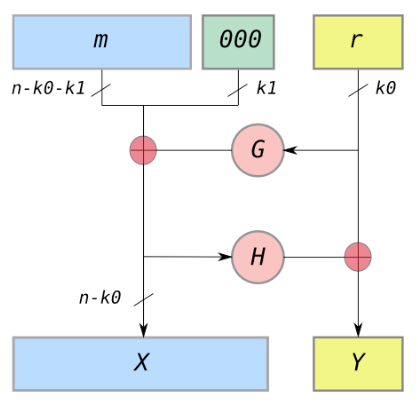
\includegraphics[scale=0.5]{img/img33.png}
\end{center}
\textbf{Encryption :} apply the step in the image on $m...$ then $c = (X\parallel Y)^e \mod n$\\
\textbf{Decryption :} $(X \parallel Y) = c^d \mod n$, then applies the step backward to recover $m$.\\
We consider the message $m$ has $n - k_0 - k_1$ bits where $n$ is the number of bits of the modulo, $k_1$ the number of bits of padding and $k_0$ the number of bits of $r$ which is a random value making the scheme probabilistic. $G$ and $H$ are hash function, if they behave as random oracle then the scheme is shown to be IND-CCA secure..\\
RSA-OAEP prevents that an adversary recovers any portion of the plaintext without being able to inver RSA.\\

The other scheme is RSA-KEM (key encapsulation method), it is an hybrid encryption, the secret (symmetric) key can be chosen at random, it will then be encapsulated with public key method.\\ 
A encapsulate the key by : choosing a random $m$ of the same bit size as \textcolor{ao}{$n$}, encrypting $c = m^{\textcolor{ao}{e}} \mod \textcolor{ao}{n}$, sending $c$ to B and then computing $k =$ hash($m$).\\
B decapsulate by recovering $m = c^{\textcolor{red}{d}} \mod \textcolor{ao}{n}$ and computing $k =$ hash($m$).\\
$k$ is the key used for the symmetric encryption.

\subsection{RSA for authenticity}
The "textbook signature" ($(m,s)$ with $s = m^{\textcolor{red}{d}} \mod \textcolor{ao}{n}$ then check if $m = s^{\textcolor{ao}{e}}$)  is susceptible to forgery attack exploiting the multiplicative structure :
\begin{itemize}
\item Ask for the signature of $m_1 : s_1 = m_1^d \mod n$
\item Ask for the signature of $m_2 : s_2 = m_2^d \mod n$
\item Comput $m_3 = m_1 \times m_2 \mod n$ and $s_3 = s_1 \times s_2 \mod n$
\item $(m_3,s_3)$ will pass verification $m_3 \equiv m_1 m_2 \equiv s_1^e s_2^e \equiv s_3^e \mod n$
\end{itemize}
Also the textbook signature only allow to sign $m$ as long as $s$. A solution against this type of attack is the use of hash function on $m : h(m)^d \mod n$. Then finding the $m_3$ correponding to $s_1 \times s_2$ would to find the preimage of the hash function.\\

If the message is short enough, it can be embeded in the signature, it's called \emph{RSA with recovery}.\\
Let $R(m) \rightarrow m'$ be a redundancy function from message space $M$ to range $\mathcal{R} \subset \mathbb{Z}_n$.\\ 
\textbf{Signature :} Compute $m' = R(m)$ then send $s = (m')^{\textcolor{red}{d}} \mod \textcolor{ao}{n}$\\
\textbf{Verification :} recover $m' = s^{\textcolor{ao}{e}} \mod \textcolor{ao}{n}$, then if $m' \in \mathcal{R}$, return $m = R^{-1}(m')$ and accept it, otherwise reject it. This scheme is not used much in practice.

Another scheme use for authenticity is RSA with full-domain hashing. The idea is to sign message of any length by putting them through a hash function first. As mentionned before it also solve the problem of forgery attacks if the hash function has preimage resistance. Let $h$ be an extendable output function (or take an old styme hash function and use MGF1 - mask generating function).\\
\textbf{Signature :} Compute $h = H(m)$ so that $h$ has the same bit size as \textcolor{ao}{$n$} then send $(m,s)$ with $s = h^{\textcolor{red}{d}} \mod \textcolor{ao}{n}$\\
\textbf{Verification : } Compute $h = H(m)$ like above then check $h \stackrel{?}{=} s^{\textcolor{ao}{e}} \mod \textcolor{ao}{n}$\\

A last scheme is RSA with PSS (probabilistic signature scheme). In the image below, \emph{padding} 1 and 2 are a fixed specified number of bits, \emph{salt} is a random value different each times and \emph{MGF} is a hash function, more precisely a mask generating function.
\begin{center}
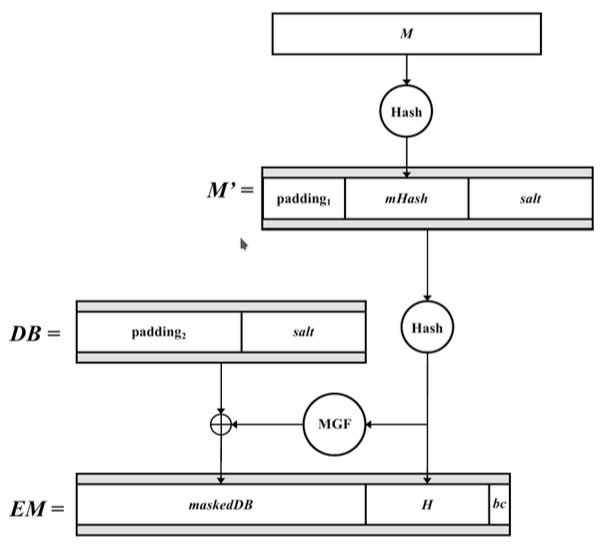
\includegraphics[scale=0.5]{img/img34.png}
\end{center}
\textbf{Signature :} From $m$ and random $salt$ comput $EM$ then send $(m,s)$ with $s = (EM)^{\textcolor{red}{d}} \mod \textcolor{ao}{n}$\\
\textbf{Verification :} Recover $EM = s^{\textcolor{ao}{e}} \mod \textcolor{ao}{n}$, recover $salt$ by using the $H$ part of $EM$ in MGF then XOR it with \textit{maskedDB}, compute $M'$ from $M$ then check $H \stackrel{?}{=} $ hash$(M')$ to see if the salt found is correct.

\subsection{RSA implementation}
A first problem is to find large prime number, the number of prime up to large $n$ is $\pi(n) \sim \dfrac{n}{\ln n}$ (the average prime gap for number of $b$ bits is about $b \ln 2$). The usual recipe is to draw a random number $n$, test co-primality with the first few primes 2,3,5,...  then test something called \emph{pseudo}-primality with for example Miller-Rabin. If $n$ doesn't pass the test then increment $n$ and repeat.\\

The different algo often requiered to do exponentiation here is a method to do it using square and multiply. To compute $a^e \mod n$ we can write the exponent in binary and apply the \textbf{square and multiply} algorithm. We also reduce the numbers modulo $n$ as we compute. (cet algo est pas très clair mais j'ai pas l'impression qu'on l'a utilisé)

Decryption and signature generation can be speeded up by keeping \textcolor{red}{$p$} and \textcolor{red}{$q$} and using the chinese remainder theorem.\\
Instead of computing $m = c^d \mod n$ comput $m_p = c^d \mod p = c^{d \mod (p-1)} \mod p$ and $m_q = c^d \mod q = c^{d \mod (q-1)} \mod q$. Then recombine $m = (m_q - m_p)(p^{-1} \mod q)p = m_p$.

To remember:
\begin{itemize}
\item How a public/private key pair is generated.
\item How to do textbook encryption, why it works (mathematically) and why it is not secure.
\item How to securely use RSA for encryption and key encapsulation.
\item How to do textbook signature, why it works (mathematically) and why it is not secure.
\item How to securely use RSA for signature.
\end{itemize}

\section{Discrete logarithm problem in $\mathbb{Z}_p^*$}
To goal of this section is to introduce the discrete logarithm (DL) problem (in the classical sense, that is, based on modular exponentiation) as well as the Diffie-Hellman (DH) problem. It then presents some of the schemes we can build on these problems.

Nowadays we don't base security on factorization problem but on logarithm problem. It's based on the fact that if we have $p$ a large prime, $g$ a generator of $\mathbb{Z}_p^*$ i.e. ${g^i \mod p : i \in \mathbb{N}} = \mathbb{Z}_p^*$, then given $A = g^a \mod p$, finding $a$ is very difficult. Finding $a$ is the discrete logarithl problem (DLP) and there are currently no known polynomial time algorithm to solve this problem.\\

%The point where i decided to add new command for \textcolor{red} and \textcolor{ao}
The \textcolor{ao}{public}-\tr{private} key pair can be generate as follows : a random integer $\tr{a} \in \mathbb{Z}_{p-1}$ is chosen privately, then we compute $\tg{A} = g^{\tr{a}} \mod p$. We now have a \tg{public} key $\tg{A}$ and a \tr{private} key $\tr{a}$.\\

\subsection{ElGamal Encryption}
The \textbf{encryption} of $m \in \mathbb{Z}_p^*$ with A's public key $\tg{A}$ : we randomly choose an integer $k \in [1,p-2]$ then compute $K = g^k \mod p$ and $c = m \tg{A}^k \mod p$\\
\textbf{Decryption} of $(K,c)$ using A's private key $\tr{a}$: compute $m = K^{-\tr{a}} c \mod p$\\
We can check that it's correct :
$$K^{-a} \equiv (g^k)^{-a} \equiv (g^a)^{-k} \equiv (A^k)^{-1} \mod p$$
$$(A^k)^{-1} c \equiv (A^k)^{-1} m(A^k) \equiv m \mod p$$
Also the first line shows how to compute the multiplicative inverse.\\

We can see $\tg{K}$ and $\tr{k}$ as an \emph{ephemeral key pair} created by the sender. $\tg{K}$  is part of the ciphertext and $\tr{k}$ is protected by the DLP. However $\tr{k}$ \textbf{must} be secret and randomly drawn independently at each encryption ! If $k$ is known then $A^k$ can be computed and $m$ recovered from $c$. Also if we use the same $k$ twice then we have $c_1 = m_1 A^k \mod p$ and $c_2 = m_2 A^k \mod p$ which means $c_1 c_2^{-1} \equiv m_1 m_1 m_2^{-1} \mod p$. It's a bit similar to what happens when we reuse a OTP.\\
ElGamal encryption relies on the DLP for security but also on the Diffie-Hellman problem.

\subsection{Diffier-Hellman problem}
If we have a large prime $p$ and $g$ a generator of $\mathbb{Z}_p^*$ i.e. ${g^i \mod p : i \in \mathbb{N}} = \mathbb{Z}_p^*$. Then given $X = g^x \mod p$ and $Y = g^y \mod p$, finding $X^y = Y^x = g^{xy} \mod p$ is fearly difficult. It's an easier problem than DLP (breaking DLP gives us the solution here but the inverse doesn't work). But still, there are currently no know polynomial time algo that solve the Diffie-Hellman problem (DHP).\\

To break ElGamal we don't need to recover $\tr{a}$ or $\tr{k}$ from $\tg{A}$ or $\tg{K}$ (DLP), we only need to recover $K^a = A^k = g^{ak} \mod p$ which is a DHP and thus a bit easier.

\subsection{Diffie-Hellman key agreement}
Here we don't directly choose the key but we use an algorithm that will give us the key, also it's an hybrid encryption. This method ensure that there is no middle man attack.\\
The domain parameter are the large prime $p$ and $g$ a generator of $\mathbb{Z}_p^*$ i.e. ${g^i \mod p : i \in \mathbb{N}} = \mathbb{Z}_p^*$. \\
A's key pair $\tg{A} = g^{\tr{a}} \mod p$\\
B's key pair $\tg{B} = g^{\tr{b}} \mod p$\\
A computes : $K_{AB} = \tg{B}^{\tr{a}} \mod p$ and $k_{AB} = \text{hash}(K_{AB})$\\
B computes : $K_{AB} = \tg{A}^{\tr{b}} \mod p$ and $k_{AB} = \text{hash}(K_{AB})$\\
Then we can use $k_{AB}$ for symmetric encryption between A and B. It work because $A^b \equiv g^{ab} \equiv B^a  (\mod p)$\\

If we want to avoid using the same long-term keys for all communications we can use \emph{ephemeral} DH key agreement :
A's long-term key pair $\tg{A} = g^{\tr{a}} \mod p$\\
B's long-term key pair $\tg{B} = g^{\tr{b}} \mod p$\\
\\
A randomly chooses $\tr{e}$, sends $\tg{E} = g^{\tr{e}} \mod p$ along with sign$_{\tr{a}} (\tg{E})$\\
B randomly chooses $\tr{f}$, sends $\tg{F} = g^{\tr{f}} \mod p$ along with sign$_{\tr{b}} (\tg{F})$\\
A checks B's signature with $\tg{B}$ and computes $K_{AB} = \tg{F}^{\tr{e}} \mod p$ and $k_{AB} = \text{hash}(K_{AB})$\\
B checks A's signature with $\tg{A}$ and computes $K_{AB} = \tg{E}^{\tr{f}} \mod p$ and $k_{AB} = \text{hash}(K_{AB})$\\
We can use $k_{AB}$ for symmetric encryption between A and B. $e$ and $f$ are the ephemeral private keys, $E$ and $F$ are the ephemeral piblic keys. The long term key pairs are used to ensure that $E$ and $F$ are from the right person.

\subsection{ElGamal signature}
\textbf{Signature} of $m \in \mathbb{Z}_2^*$ by sender A's private key $\tr{a}$:
\begin{itemize}
\item compute $h =$ hash$(m)$
\item choose randomly an integer $k \in [1,p-2]$
\item compute $r = g^k \mod p$
\item compute $s = k^{-1} (h- \tr{a}r) \mod (p-1)$, if $s=0$ restart with new $k$
\item send $(r,s)$ along with $m$.
\end{itemize}
$\tr{k}$ and $\tg{r}$ can be viewed as an ephemeral key pair.\\
\\
\textbf{Verification} of signature $(r,s)$ on $m$ with A's public key $\tg{A}$ is done by computing $h =$ hash$(m)$ then checking $\tg{A}^r r^s \stackrel{?}{\equiv} g^h \mod p$\\

It works :
$$\begin{array}{rl}
A^r r^s & \equiv (g^a)^r (g^k)^s\\
& \equiv g^{ar + ks \mod (p-1)} \\
& \equiv g^{ar + kk^{-1} (h-ar) \mod (p-1)} \\
& \equiv g^{ar + h-ar \mod (p-1)} \\
& \equiv g^h \mod p
\end{array}$$

As mentioned before $\tr{k}$ can be seen as the private part of the ephemeral key pair $(r,s)$ created by the signer and $\tr{k}$ is protected by the DLP. However $k$ \textbf{must} be secret and randomly drawn independently at each encryption. If $k$ is known then $\tr{a}$ can be recovered from $s$. If $k$ is repeated to sign messages with hashes $h_1 \neq h_2$ then $s_1 - s_2 \equiv k^{-1} (h_1 - ar) - k^{-1}(h_2 - ar) \equiv k^{-1}(h_1 - h_2) \mod (p-1)$ and we can recover $k$ then $\tr{a}$ from $s_1$ or $s_2$

There is another scheme DSA which is a compact variant of ElGamal but it's more for our information.

\subsection{Schnorr signature}
\textbf{Signature} of $m \in \mathbb{Z}_2^*$ with A's priavte key $\tr{a}$ :
\begin{itemize}
\item choose randomly an integer $k \in [1,p-2]$
\item compute $r = g^k \mod p$
\item compute $e = hash(r \parallel m)$
\item compute $s = k - e\tr{a} \mod (p-1)$
\item send $(s,e$ along with $m$.
\end{itemize}

\textbf{Verification} of signature $(s,e)$ on $m$ with A's public key $\tg{A}$ is done by computing $r' = g^s \tg{A}^e \mod p$, computing $e' =$ hash$(r' \parallel m)$ then checking $e' \stackrel{?}{=} e$ which in fact check if $r' \stackrel{?}{=} r$.\\

The verification works because $r' = g^s A^e = g^{k-ea} g^{ae} = g^k = r$.

Note : on the various scheme presented before sometimes in the signature we use $\mod p$ and sometimes $\mod (p-1)$, we use the latter when the $s$ is gonna be used in the exponent for the verification.
 
To remember:
\begin{itemize}
\item What are the DL and DH problems and how they relate to each other.
\item Why ElGamal encryption works and what are the properties k must satisfy.
\item Why Diffie-Hellman key exchange works.
\item Why ElGamal signature works and what are the properties k must satisfy.
\item Why Schnorr signature works and what are the properties k must satisfy.
\end{itemize}

\section{Security of the discrete logarithm problem}
The goal of this section is to transition to other types of discrete logarithm (DL) problems. We focus on the inherent limits of security of the DL problem.

There is a generic method to solve the DLP called baby-steps giant-step, this method work for any group but the developpement is more intuitive for a group \textcolor{magenta}{$\mathbb{Z}_p^*$} where the operator $[n]$ is \textcolor{magenta}{$^n$}.\\

So for any group $G$ \textcolor{magenta}{($\mathbb{Z}_p^*$)} the DLP is : given $A = [a]g$ \textcolor{magenta}{($A = g^a \mod p$)}, find $a$.\\
\\
Let $N = |G|$ \textcolor{magenta}{($N = |\mathbb{Z}_p^* |$)} and $g$ be a generator of the group.
\begin{itemize}
\item Let $m \approx \sqrt{N}$ and suppose that $a = a_0+a_1 m$ with $a_0 , a_1 < m$
\item $A = [a_0 + a_1 m]g \Leftrightarrow A \circ [-a_1 m]g = [a_0]g$ \textcolor{magenta}{($A \equiv g^{a_0 + a_1 m} \mod p \Leftrightarrow A g^{a_1 m} \equiv g^{a_0} \mod p$)}
\item For $i=0$ to $m-1$ sequentially (\emph{baby steps}) : compute and store $(i,[i]g)$ \textcolor{magenta}{($(i,g^i)$)}, i.e apply $\circ g$ \textcolor{magenta}{(mutliply by $g$)} at each steps
\item For $j = 0$ to $m-1$ sequentially (\emph{giantss steps}) : compute $A \circ [-jm]g \textcolor{magenta}{(Ag^{-jm})}$, i.e apply $\circ [-m]g$ \textcolor{magenta}{(multiply by $g^{-m}$)} at each steps, if $A \circ [-jm]g = [i]g \textcolor{magenta}{(A g^{-jm} = g^i)} $ then $a = i+jm$ and exit.
\end{itemize}
The time and memory needed are $O(\sqrt{N})$. If the size of the group can be decomposed in prime factors : $N = |G| = \prod\limits_i p_i^{e_i}$, then we can solve the DLP in time
$$O\left( \sum\limits_i e_i (\log N + \sqrt{p_i}) \right)$$
2 conditions are \textbf{necessary} (but no sufficient) for the DLP to be hard : the size of the group should be $\approx 2^{2s}$ for security strength $s$ and the size of the group should be prime.


To remember :
\begin{itemize}
\item What are the inherent security limits of the DL problem given the size of the group.
\item The security does not depend only on the size of the group but also on the representation of the elements. For instance, the DL problem over a modular additive group is trivial to solve.
\end{itemize}

\section{Elliptic curve cryptography}
This section aims at introducing elliptic curves over finite fields and to show how they can be used in cryptography. We make a tour of the different forms of elliptic curves that are used in cryptography nowadays (Weierstrass, Montgomery, Edwards).

To remember:
\begin{itemize}
\item A group law can be defined over an elliptic curve. The discrete logarithm problem can be generalized to this group, called the elliptic curve discrete logarithm (ECDL) problem.
\item Unless the curve admits non-general properties, the fastest known way to solve the ECDL problem is to solve it generically (e.g., using the baby-step-giant-step algorithm).
\item Schemes based on the DL problem can be translated into their elliptic curve equivalent by using the group notation. Hence, elliptic curves can be used to do public-key encryption, key exchange and signature.
\end{itemize}


\section{Protocol}
The goal of this section is to present simple identification protocols based on the DL (or ECDL) problem and to show how this can be generalized in a way that naturally leads to the Schnorr signature scheme.

To remember:
\begin{itemize}
\item What is an identification protocol, how to prevent an adversary to impersonate, how to prevent the prover to cheat.
\item How to make an interactive protocol non-interactive.
\item How to explain the Schnorr signature scheme from the Schnorr identification scheme.
\end{itemize}

\end{document}